%% Use the option review to obtain double line spacing
%% \documentclass[authoryear,preprint,review,12pt]{elsarticle}
\documentclass[final,3p,times,twocolumn]{elsarticle}

% \usepackage[table]{xcolor}
% %% the amssymb package provides various useful mathematical symbols
% \usepackage{amssymb}

% %% the amsthm package provides extended theorem environments
% \usepackage{amsthm}

%% amsmath for math environment
\usepackage{amsmath}

% \declaremathoperator*{\argmin}{arg\,min}
% \declaremathoperator*{\argmax}{arg\,max}
% \declaremathoperator*{\sign}{sign}
% \declaremathoperator*{\infspie}{inf}


% % to break equation
% %\usepackage{mathpazo}
% %\usepackage{mathptmx}
% %\usepackage[mathpazo]{flexisym}
% %\usepackage{breqn}

%% for clever reference
\usepackage{cleveref}

%% color package
\usepackage{color}

%% figure package
\usepackage{epsf,graphicx}
\usepackage{epstopdf}
\usepackage{subfigure}	
\usepackage{transparent}

% %% new environment to have some indent inside enumerate environment
% \usepackage{enumitem}

%% to create acronym for proper glossary
\usepackage{acro}

% %% To number the line in the article
% \usepackage{lineno}

%% Environment to include table with notes
\usepackage{array}
\usepackage{threeparttable}
\usepackage{booktabs}
\usepackage{multirow}
% \usepackage{siunitx}

% %% In order to change size of margin
% \usepackage{geometry}
% \usepackage{changepage}
% \usepackage{lscape}

%% Colorpackage for table
\usepackage{colortbl}
\usepackage{tabularx}
\usepackage{arydshln}

%% To use URL referencing
\usepackage{url}
%\usepackage[hidelinks]{hyperref}

%% In order to draw some graphs
\usepackage{tikz,xifthen}
\usepackage{tikz-qtree}
\usetikzlibrary{decorations.pathmorphing} % noisy shapes
\usetikzlibrary{fit}					% fitting shapes to coordinates
\usetikzlibrary{backgrounds}	% drawing the background after the foreground
\usetikzlibrary{shapes,arrows,shadows}
\usetikzlibrary{calc,decorations.pathreplacing,decorations.markings,positioning}
\usetikzlibrary{snakes,decorations.text,shapes,patterns}
%\usepackage{scalefnt,lmodern,booktabs}

%% Paxkage for cross and tick symbols
\usepackage{pifont}
\newcommand{\cmark}{\color{green!60!black!80}\ding{51}}
\newcommand{\mmark}{{\color{green!60!black!80}\ding{51}}$^{!}$}
\newcommand{\xmark}{\color{red!60!black!80}\ding{55}}
\newcommand{\cmarksmall}{\color{green!60!black!80}\ding{51}}
\newcommand{\mmarksmall}{{\color{green!60!black!80}\ding{51}}$^{!}$}
\newcommand{\xmarksmall}{\color{red!60!black!80}\ding{55}}
\newcommand{\Conv}{\mathop{\scalebox{1.5}{\raisebox{-0.2ex}{$\ast$}}}}%

\definecolor{autoGuided}{rgb}{ 0.3765    0.7294    0.9412}
\newcommand{\autoGuidedColor}{(light-Blue)}
\definecolor{fullyAuto}{rgb}{ 0.0941    0.3843    0.6627}
\newcommand{\fullyAutoColor}{(dark-blue)}
\definecolor{semiAuto}{rgb}{ 0.0784    0.5059    0.1686}
\newcommand{\semiAutoColor}{(light-green)}
\definecolor{fullyGuided}{rgb}{ 0.4275    0.6902    0.3176}
\newcommand{\fullyGuidedColor}{(dark-green)}

% \DeclareSIUnit\ppm{ppm}
% \DeclareSIUnit\px{px}

\usepackage{ltxtable}
\usepackage{listings}
\usepackage{color}
\usepackage[toc]{appendix}
 
\definecolor{codegreen}{rgb}{0,0.6,0}
\definecolor{codegray}{rgb}{0.5,0.5,0.5}
\definecolor{codepurple}{rgb}{0.58,0,0.82}
\definecolor{backcolour}{rgb}{0.95,0.95,0.92}
 
% \lstdefinestyle{mystyle}{
%     backgroundcolor=\color{backcolour},   
%     commentstyle=\color{codegreen},
%     keywordstyle=\color{magenta},
%     numberstyle=\tiny\color{codegray},
%     stringstyle=\color{codepurple},
%     basicstyle=\footnotesize,
%     breakatwhitespace=false,         
%     breaklines=true,                 
%     captionpos=b,                    
%     keepspaces=true,                 
%     numbers=left,                    
%     numbersep=5pt,                  
%     showspaces=false,                
%     showstringspaces=false,
%     showtabs=false,                  
%     tabsize=2
% }
 
% \lstset{style=mystyle}
\usepackage{setspace}    
%\acrodef{cap}[CaP]{prostate cancer}
\DeclareAcronym{cap}{
short = CaP,
long = prostate cancer
}
\DeclareAcronym{pirads}{
short = PI-RADS,
long = Prostate imaging reporting and data system
}
%\acrodef{cade}[CADe]{computer-aided detection}
\DeclareAcronym{cade}{
short = CADe,
long = computer-aided detection
}
%\acrodef{cadx}[CADx]{computer-aided diagnosis}
\DeclareAcronym{cadx}{
short = CADx,
long = computer-aided diagnosis
}
\DeclareAcronym{lm}{
short = LM, 
long = Leung-Malik set
}
%\acrodef{us}[US]{ultrasound}
\DeclareAcronym{us}{
short = UTS,
long = ultrasound
}
%\acrodef{ct}[CT]{computer tomography}
\DeclareAcronym{ct}{
short = CT,
long = computer tomography
}
%\acrodef{cad}[CAD]{computer-aided detection and diagnosis}
\DeclareAcronym{cad}{
short = CAD,
long = computer-aided detection and diagnosis
}
%\acrodef{mri}[MRI]{magnetic resonance imaging}
\DeclareAcronym{mri}{
short = MRI,
long = magnetic resonance imaging
}
%\acrodef{nmr}[NMR]{nuclear magnetic resonance}
\DeclareAcronym{nmr}{
short = NMR,
long = nuclear magnetic resonance
}

\DeclareAcronym{omp}{
  short = OMP,
  long =  orthogonal matching pursuit 
}
\DeclareAcronym{adb}{
  short = AdB, 
  long = AdaBoost
}
\DeclareAcronym{gb}{
  short = GB, 
  long = Gradient Boosting
}

\DeclareAcronym{mp}{
  short = MP,
  long =  Matching Pursuit 
}
%\acrodef{t2w}[T$_2$-W]{T$_2$ Weighted}
\DeclareAcronym{t2w}{
short = T$_2$-W,
long = T$_2$ Weighted
}
%\acrodef{dce}[DCE]{dynamic contrast-enhanced}
\DeclareAcronym{dce}{
short = DCE,
long = dynamic contrast-enhanced
}
%\acrodef{dw}[DW]{diffusion weighted}
\DeclareAcronym{dw}{
short = DW,
long = diffusion weighted
}
%\acrodef{mrsi}[MRSI]{magnetic resonance spectroscopy imaging}
\DeclareAcronym{mrsi}{
short = MRSI,
long = magnetic resonance spectroscopy imaging
}
%\acrodef{bph}[BPH]{benign prostatic hyperplasia}
\DeclareAcronym{bph}{
short = BPH,
long = benign prostatic hyperplasia
}
%\acrodef{pz}[PZ]{peripheral zone}
\DeclareAcronym{pz}{
short = PZ,
long = peripheral zone
}
%\acrodef{cz}[CZ]{central zone}

\DeclareAcronym{mpmri}{
short = mp-MRI,
long = multiparametric \ac{mri}
}
\DeclareAcronym{cz}{
short = CZ,
long = central zone
}
%\acrodef{tz}[TZ]{transitional zone}
\DeclareAcronym{tz}{
short = TZ,
long = transitional zone
}
%\acrodef{cg}[CG]{central gland}
\DeclareAcronym{cg}{
short = CG,
long = central gland
}
%\acrodef{psa}[PSA]{prostate-specific antigen}
\DeclareAcronym{psa}{
short = PSA,
long = prostate-specific antigen
}
%\acrodef{trus}[TRUS]{transrectal ultrasound}
\DeclareAcronym{trus}{
short = TRUS,
long = transrectal ultrasound
}
%\acrodef{tr}[TR]{repetition time}
\DeclareAcronym{tr}{
short = TR,
long = repetition time
}
%\acrodef{te}[TE]{echo time}
\DeclareAcronym{te}{
short = TE,
long = echo time
}
%\acrodef{si}[SI]{signal intensity}
\DeclareAcronym{si}{
short = SI,
long = signal intensity
}
%\acrodef{ees}[EES]{extravascular-extracellular space}
\DeclareAcronym{ees}{
short = EES,
long = extravascular-extracellular space
}
%\acrodef{t1w}[T$_1$-W]{T$_1$ Weighted}
\DeclareAcronym{t1w}{
short = T$_1$-W,
long = T$_1$ Weighted
}
%\acrodef{fse}[FSE]{Fast Spin-Echo}
\DeclareAcronym{fse}{
short = FSE,
long = Fast Spin-Echo
}
%\acrodef{adc}[ADC]{Apparent Diffusion Coeffient}
\DeclareAcronym{adc}{
short = ADC,
long = apparent diffusion coefficient
}
%\acrodef{roi}[ROI]{region of interest}
\DeclareAcronym{roi}{
short = ROI,
long = region of interest
}
%\acrodef{cse}[CSE]{chemical shift effect}
\DeclareAcronym{cse}{
short = CSE,
long = chemical shift effect
}
%\acrodef{snr}[SNR]{signal-to-noise}
\DeclareAcronym{snr}{
short = SNR,
long = signal-to-noise
}
\DeclareAcronym{se}{
short = SE, 
long = sensitivity
}
\DeclareAcronym{sp}{
short = SP, 
long = specificity
}
%\acrodef{gs}[GS]{Gleason score}
\DeclareAcronym{gs}{
short = GS,
long = Gleason score
}
%\acrodef{ersspc}[ERSSPC]{European Randomized Study of Screening for Prostate Cancer}
\DeclareAcronym{ersspc}{
short = ERSSPC,
long = European randomized study of screening for prostate cancer
}
%\acrodef{plco}[PLCO]{Prostate, Lung, Colorectal and Ovarian}
\DeclareAcronym{plco}{
short = PLCO,
long = prostate lung colorectal and ovarian
}
%\acrodef{fig}[Fig.]{figure}
\DeclareAcronym{fig}{
short = Fig.,
long = figure,
class = latex
}
\DeclareAcronym{tab}{
short = Table,
long = table,
class = latex
}
\DeclareAcronym{eq}{
short = Eq.,
long = equation,
class = latex
}
\DeclareAcronym{sec}{
short = Sect.,
long = section,
class = latex
}
\DeclareAcronym{chp}{
short = Chap.,
long = Chapter,
class = latex
}

\DeclareAcronym{fov}{
short = FOV,
long = field of view
}
\DeclareAcronym{dwt}{
short = DWT,
long = discrete wavelet transform
}
\DeclareAcronym{dwst}{
short = DWST,
long = discrete wavelet squared transform
}
\DeclareAcronym{map}{
short = MAP,
long = maximum \textit{a posteriori}
}
\DeclareAcronym{ml}{
short = ML,
long = maximum likelihood
}
\DeclareAcronym{mle}{
short = MLE,
long = maximum likelihood estimation
}
\DeclareAcronym{mrf}{
short = MRF,
long = Markov random field
}
\DeclareAcronym{itk}{
short = ITK,
long = Insight Segmentation and Registration Toolkit
}
\DeclareAcronym{es}{
short = ES,
long = Evolution Strategy
}
\DeclareAcronym{scf}{
short = SCF,
long = sparse coded features
}
\DeclareAcronym{bow}{
short = BoW,
long = bag of words
}
\DeclareAcronym{pdf}{
short = PDF,
long = probability density function
}
\DeclareAcronym{gscale}{
short = \textit{g}-scale,
long = generalized scale
}
\DeclareAcronym{aif}{
short = AIF,
long = arterial input function
}
\DeclareAcronym{svd}{
short = SVD,
long = singular value decomposition
}
\DeclareAcronym{mse}{
short = MSE,
long = mean squared error
}
\DeclareAcronym{mi}{
short = MI,
long = mutual information
}
\DeclareAcronym{mantra}{
short = MANTRA,
long = multi-attribute non-initializing texture reconstruction based active shape model
}
\DeclareAcronym{asm}{
short = ASM,
long = active shape model
}
\DeclareAcronym{pca}{
short = PCA,
long = principal components analysis
}
\DeclareAcronym{weritas}{
short = WERITAS,
long = weighted ensemble of regional image textures for active shape model segmentation
}
\DeclareAcronym{staple}{
short = STAPLE,
long = simultaneous truth and performance level estimation
}
\DeclareAcronym{lda}{
short = LDA,
long = linear discriminant analysis
}
\DeclareAcronym{lbp}{
short = LBP,
long = local binary pattern
}
\DeclareAcronym{tps}{
short = TPS,
long = thin plate spline
}
\DeclareAcronym{acm}{
short = ACM,
long = active contour model
}
\DeclareAcronym{cmi}{
short = CMI,
long = combined mutual information
}
\DeclareAcronym{svm}{
short = SVM,
long = support vector machines
}
\DeclareAcronym{rvm}{
short = RVM,
long = relevant vector machine
}
\DeclareAcronym{rbf}{
short = RBF,
long = radial basis function
}
\DeclareAcronym{knn}{
short = $k$-NN,
long = $k$-nearest neighbour
}
\DeclareAcronym{nn}{
short = NN,
long = neareast neighbour
}
\DeclareAcronym{dct}{
short = DCT,
long = discrete cosine transform
}
\DeclareAcronym{hog}{
short = HOG,
long = histogram of oriented gradient
}
\DeclareAcronym{dft}{
short = DFT,
long = discrete fourier transform
}
\DeclareAcronym{us1}{
short = US,
long = under-sampling
}
\DeclareAcronym{os}{
short = OS,
long = over-sampling
}
\DeclareAcronym{ros}{
short = ROS,
long = random-over-sampling
}
\DeclareAcronym{rus}{
short = RUS,
long = random-under-sampling
}
\DeclareAcronym{nm}{
short = NM,
long = nearmiss
}
\DeclareAcronym{nm3}{
short = NM-3,
long = nearmiss-3
}
\DeclareAcronym{nm2}{
short = NM-2,
long = nearmiss-2
}
\DeclareAcronym{nm1}{
short = NM-1,
long = nearmiss-1
}
\DeclareAcronym{iht}{
short = IHT,
long = instance-hardness-threshold
}
\DeclareAcronym{smote}{
short = SMOTE,
long = synthetic minority over-sampling techniques
}
\DeclareAcronym{smoteb1}{
short = SMOTE-b1,
long = SMOTE-borderline1
}
\DeclareAcronym{smoteb2}{
short = SMOTE-b2,
long = SMOTE-borderline2
}
\DeclareAcronym{mrmr}{
short = mRMR,
long = minimum redundancy maximum relevance
}
\DeclareAcronym{lle}{
short = LLE,
long = locally linear embedding
}
\DeclareAcronym{ica}{
short = ICA,
long = independent components analysis
}
\DeclareAcronym{qda}{
short = QDA,
long = quadratic discriminant analysis
}
\DeclareAcronym{id3}{
short = ID3,
long = iterative dichotomiser 3
}
\DeclareAcronym{cart}{
short = CART,
long = classification and regression tree
}
\DeclareAcronym{bagging}{
short = bagging,
long = bootsrap aggregating
}
\DeclareAcronym{loo}{
short = LOOCV,
long = leave-one-out cross-validation
}
\DeclareAcronym{lopo}{
short = LOPO CV,
long = leave-one-patient-out cross-validation
}

\DeclareAcronym{kcv}{
short = $k$-CV,
long = $k$-fold cross-validation
}
\DeclareAcronym{roc}{
short = ROC,
long = receiver operating characteristic
}
\DeclareAcronym{froc}{
short = FROC,
long = free-response receiver operating characteristic
}
\DeclareAcronym{auc}{
short = AUC,
long = area under the curve
}
\DeclareAcronym{rmse}{
short = RMSD,
long = root-mean-square deviation
}
\DeclareAcronym{rms}{
  short = RMS,
  long = root mean square
}
\DeclareAcronym{srsf}{
  short = SRSF,
  long =  square-root slope function
}
\DeclareAcronym{pun}{
short = PUN,
long = phenomenological universalities
}
\DeclareAcronym{etl}{
short = ETL,
long = echo train ength
}

\DeclareAcronym{rf}{
short = RF,
long = random forest
}
\DeclareAcronym{dna}{
short = DNA,
long = deoxyribonucleic acid
}

\DeclareAcronym{glcm}{
short = GLCM,
long = gray-level co-occurence matrix
}

\DeclareAcronym{iccvb}{
short = I2Cvb,
long = initiative for collaborative computer vision benchmarking
}

\DeclareAcronym{mloss}{
short = MLOSS 2015,
long = machine learning open source software 2015
}

\DeclareAcronym{ci}{
short = CI,
long = continuous integration
}

\DeclareAcronym{cern}{
short = CERN,
long = european organization for nuclear research
}

\DeclareAcronym{doi}{
short = DOI,
long = digital object identifier
}

\DeclareAcronym{pd}{
short = PD,
long = proton density
}

\DeclareAcronym{anova}{
short = ANOVA,
long = analysis of variance
}

\DeclareAcronym{gt}{
short = GT,
long = ground truth
}

\begin{document}

\begin{frontmatter}

  \journal{Computerized Medical Imaging and Graphics}

  \title{Computer-aided detection and diagnosis using Multi-modal MRI for
    prostate cancer detection}

  \author[label1]{G.~Lemaitre}
  \author[label2]{F.~M\'eriaudeau}
  \author[label3]{R.~Mart\'i}

  \address[label1]{Parietal team, Inria, CEA, Universit\'e Paris-Saclay, 1 Rue
    Honor\'e d’Estienne d’Orves, 91120 Palaiseau}
  \address[label2]{LE2I UMR6306, CNRS, Arts et M\'etiers, Univ. Bourgogne
    Franche-Comt\'e, 12 rue de la Fonderie, 71200 Le Creusot}
  \address[label3]{ViCOROB, Universitat de Girona, Campus Montilivi, Edifici P4,
    17071 Girona}

  \begin{abstract}
    Study the advantages of using multi-modal imagery in computer-aided
    detection and diagnosis systems for prostate cancer with special attention to
    pre-processing and data-balancing stages of a CaD.  A multi modal MR volumes
    including T2W-MRI, DCE-MRI, DW-MRI and MRSI with accompanying ground-truth were
    acquired from 17 patients. The proposed CaD system to conduct this study
    consists of pre-processing, segmentation, feature detection, data balancing,
    feature extraction and classification; and all results are cross-validated
    using leave one patient out strategy.  The usage of multi-modal information to
    the CaD system increases the area under the curve from $0.666\pm0.15$ up to
    $0.836\pm0.083$, showing a better and more stable results.  The study using the
    proposed framework shows that T2W-MRI is necessary to obtain satisfactory
    results however better results are obtained when combined with other
    modalities.
  \end{abstract}

  \begin{keyword}
    Computer-aided detection \sep prostate cancer \sep multi-parametric MRI\sep
    feature engineering
  \end{keyword}


\end{frontmatter}



\section{Introduction}

\Ac{cap} is the second most frequently diagnosed cancer in men, accounting for
899,000 cases and leading to 258,100 deaths per
year~\citep{ferlay2010estimates}. Early detection, diagnosis and accurate risk
assessment play a major role in patient treatment. In this regard,
Hambrock\,\emph{et~al.}\,\cite{Hambrock2013} explore the idea of incorporating
\ac{cad} systems to assist radiologists in their clinical practice. They show
that radiologists assisted with \ac{cad} for \ac{cap} detection and diagnosis
improve their screening performance, especially for inexperienced radiologists,
leveling up their performance to the senior radiologists expertise.

Despite recent advances, \ac{cap}-\ac{cad} remains a young technology mainly
because it is based on \ac{mri}~\cite{Hegde2013}. The two main challenges in
\ac{cap}-\ac{cad} systems, as pointed by the \ac{pirads} Steering Committee
are: (i) improving the detection of clinically significant \ac{cap} and (ii)
increasing confidence in benign or dormant cases to avoid unnecessary invasive
medical exams~\citep{weinreb2016pi}.

Lemaitre\,\emph{et~al.}\,\cite{lemaitre2015computer} provides an
overview and a taxonomy of the developed \acs{cad} systems for \ac{cap}
detection and diagnosis based on \ac{mri} modalities. As a conclusion, the
following shortcomings have been drawn: (i) not a single study used all available
\ac{mri} modalities, (ii) little attention has been granted to data
normalization, (iii) features have usually been extracted using solely 2D
information, and (iv) the problem of data balancing has never been
investigated. We refer the reader to~\cite{lemaitre2015computer} for a detailed
review of the previous work related to \ac{mpmri} \ac{cad} for prostate cancer
detection.

Therefore, we here propose a \ac{mpmri} \ac{cad} framework using all available
\ac{mri} modalities, as depicted in \acs{fig}\,\ref{fig:wkfcad}. In addition,
feature extracted will take advantage of the 3D information of the data
acquired. Our framework is also incorporating a data balancing step to reduce
the classification bias introduce during the learning phase.

The rest of this document is structured as follows:
\acs{sec}\,\ref{sec:materials_and_methods} details each step of our \ac{mpmri}
\ac{cad} system while \acs{sec}\,\ref{sec:experiments} reports a set of
experiments to give insights about each of these steps. Finally,
\ac{sec}\,\ref{sec:conclusion} concludes this work with a discussion and give
avenues for future research.

\section{Materials and Methods}\label{sec:materials_and_methods}

We investigate here the different steps of the \ac{cad} for \ac{cap} pipeline
presented in \acs{fig}\,\ref{fig:wkfcad}. Indeed, this pipeline is
subdivided into 2 steps: (i) image regularization and (ii) \ac{cadx}. The image
regularization covers the segmentation of the prostate organ in the
different modalities and their realignment. The \ac{cadx} step is a regular
classification pipeline in which features are detected, balanced, selected, and
finally classified. The following sections go into details in each of these
steps.

\begin{figure}
  \centering
  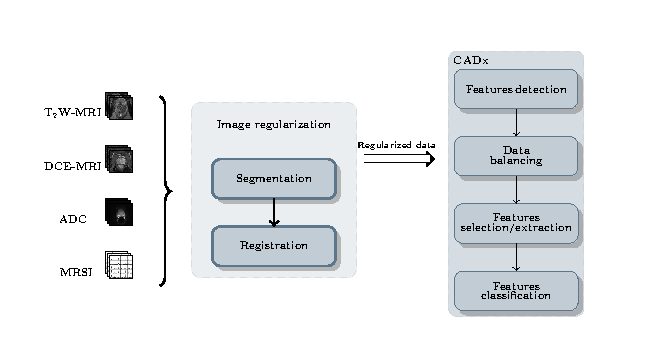
\includegraphics[width=1.0\linewidth]{./images/cad/wkfcad.pdf}
  \caption{\textbf{Our proposed \ac{mpmri} \ac{cad} framework for prostate cancer
    detection.} The \ac{mpmri} modalities are first regularized by segmenting
  the prostate organ and registering it. The second step follows a common
  classification pipeline by engineering features, balancing samples depending of
  the class occurrences, selecting features, and finally train and test a machine
  learning model. This model is evaluated through a cross-validation scheme.}
  \label{fig:wkfcad}
\end{figure}

\subsection{Segmentation and registration}

We used the manual segmentation provided by our radiologists (prostate gland,
cancerous regions, and prostate regions). In addition, we applied different
registration methods to align the volumes from the different modalities: (i)
the patient motion during the \ac{dce}-\ac{mri} acquisition, (ii) the patient
motion between the \ac{t2w}-\ac{mri} and the \ac{dce}-\ac{mri} acquisitions,
and (iii) the patient motion between the \ac{t2w}-\ac{mri} and the \ac{adc} map
acquisition.

\begin{itemize}

\item[(i)] The \ac{dce}-\ac{mri} acquisition being dynamic, some intra-patient
motions might occur during the acquisition. For each serie of this dynamic
acquisition, each 3D volume is registered to the first volume acquired to
remove the residual motion. The appearance in the \ac{dce}-\ac{mri} images,
however, varies due to the presence or not of the contrast media. Therefore,
the metric chosen to be minimized is the \ac{mi} and the geometric transform
has been set to a rigid transform. The optimization is performed using a
regular step gradient descent.

\item[(ii)] Once the intra-patient motions is corrected, \ac{t2w}-\ac{mri} and
the \ac{dce}-\ac{mri} are registered. For that matter, the prostate has been
segmented in both modalities --- \ac{t2w}-\ac{mri} and \ac{dce}-\ac{mri} --- to
create two binary masks. These 3D binary masks are subsequently
registered using the \ac{mse} metric. Unlike the previous registration, we use
a more complex geometric transform by successively finding a rigid
transformation, a coarse elastic transformation, and a fine elastic
transformation. The B-splines transformation is used as the elastic
transform. These successive transformations allow to get a good initialization
for the next transformation. The transformation parameters are inferred by
minimizing the cost function using a regular step gradient descent.

\item[(iii)] The \ac{t2w}-\ac{mri} and \ac{adc} map acquisitions are registered
using the same approach as for the registration of the \ac{t2w}-\ac{mri} and
the \ac{dce}-\ac{mri} modalities. Additionally, the \ac{cap}, \ac{pz}, and
\ac{cg} are segmented on the \ac{t2w}-\ac{mri} and thus \ac{t2w}-\ac{mri} is
used as the reference modality.

\end{itemize}

\subsection{Feature detection}

Two different types of feature are extracted due to the characteristics of the
\ac{mri} modalities used in this study. Indeed, computer vision features are
suitable for the \ac{t2w}-\ac{mri} and \ac{adc} map while specific feature
engineering, embedding domain-specific knowledge, is required for the
\ac{dce}-\ac{mri} and \ac{mrsi} data.

\subsubsection{Computer vision features}

\begin{table*}
  \caption{\textbf{Features extracted in \acs*{t2w}-\acs*{mri} and \acs*{adc}
      map.} We explore a broad set of image features characterizing
    intensity, edges, and texture.}
  \centering
  \scriptsize
  \begin{tabular}{llc}
    \toprule
    \textbf{Features} & \textbf{Parameters} & \textbf{\# dimensions} \\
    \midrule
    Intensity &  & 1 \\
    \acs*{dct} decomposition & window: \SI[product-units=repeat]{9x9x3}{\px} & 243 \\
    Kirsch filter &  & 2 \\
    Laplacian filter &  & 1 \\
    Prewitt filter &  & 3 \\
    Scharr filter &  & 3 \\
    Sobel filter &  & 3 \\
    Gabor filters & 4 frequencies $f \in [0.05, 0.25]$; 4 azimuth angles $\alpha \in [0, \pi]$; 8 elevation angles $\alpha \in [0, 2\pi]$ & 256 \\
    Phase congruency filter & 5 orientations; 6 scales & 3 \\
    Haralick filter & window: \SI[product-units=repeat]{9x9x3}{\px}; \# grey levels: 8; distance: \SI{1}{\px}; 13 directions & 169 \\
    \acs*{lbp} filter & 2 radii $r=\{1, 2\}$; 2 neighborhood sizes $N = \{8, 16\}$ & 6 \\
    \bottomrule
  \end{tabular}
  \label{tab:featureadct2w}
\end{table*}

A set of common features reported in~\cite{lemaitre2015computer} are
computed. \Acl{tab}~\ref{tab:featureadct2w} summarizes the different features
extracted with their corresponding parameters. Note that all these features are
extracted at each voxel of the volume. The voxel intensities are the most
common features encoding tumor information. However, those intensities vary
between patients. Therefore, \ac{t2w}-\ac{mri} modality is normalized using a
Rician \emph{apriori} as presented
in~\cite{lemaitre2016normalization}. \Ac{adc} coefficient is standardized as
in~\cite{Nyul1999}. The following set of filters characterizing edges are
extracted: (i) Kirsch, (ii) Laplacian, (iii) Prewitt, (iv) Scharr, (v) Sobel,
and (vi) Gabor. Apart of the Kirsh filter, other filters can be extended into
3D filter. 3D Gabor filters are not commonly used and we reused the formulation
presented in~\cite{wang2005face}. Additionally, features based on phase
congruency as proposed by Kosevi\,\emph{et~al.} are
computed~\cite{kovesi1999image}. Therefore, from a set of Log-Gabor filter
bank, the orientation image, the local weighted mean phase angle, and the phase
angle are estimated at each voxel. To characterize the local texture, both
second-order \ac{glcm}-based features~\cite{Haralick1973} and rotation
invariant and uniform \ac{lbp}~\cite{ojala2002multiresolution} are
extracted. To encode 3D information, the 13 first Haralick features are
computed for the 13 possible directions. For the same reason, the \ac{lbp}
codes are computed for the three-orthogonal-planes of each \ac{mri} volume.

\subsubsection{\acs*{dce}-\acs*{mri} features}\label{features:dce}

Two family of approaches are commonly used to extract information from the
\ac{dce}-\ac{mri} signals~\cite{lemaitre2015computer}: (i) quantitative
modeling and (ii) semi-quantitative modeling. 

\emph{Quantitative approaches} uses pharmacokinetic modeling based on a
bicompartment model, namely Brix~\cite{brix1991pharmacokinetic} and
Tofts~\cite{tofts1995quantitative} models. The parameters of the Brix model
are inferred by assuming a linear relationship between the media concentration
and the \ac{mri} signal intensity. However, this assumption has been shown to
lead to inaccurate estimations of the pharmacokinetic
parameters~\cite{heilmann2006determination}. In contrast, the Tofts model
requires the conversion of \ac{mri} signal intensity to concentration, which
becomes a non-linear relationship using a specific equation of \ac{mri}
sequences (e.g., FLASH sequence). Tofts modeling, however, is highly
complex~\cite{gliozzi2011phenomenological}. Achieving the conversion using the
non-linear approach requires the acquisition of a T$_1$ map which is not always
possible during clinical examination. Additionally, computing the parameters
require the \ac{aif} which is challenging to measure and influence the estimation.

\emph{Semi-quantitative} approaches extract a set of parameters related to a
mathematical model rather than a pharmacokinetic model, relaxing any
pharmacokinetic assumptions regarding the relationship between the \ac{mri}
signal and the contrast
agent~\cite{huisman2001accurate,gliozzi2011phenomenological}. In addition,
these methods do not require any knowledge regarding the \ac{mri} sequence or
any conversion from the signal intensity to the media concentration. However,
they present some limitations: the heuristic approach proposed
by~Huisman\,\emph{et~al.}  requires an initial estimate of the standard
deviation of the signal noise and some manual
tuning~\cite{huisman2001accurate}.

Nevertheless, all of the presented methods suffer from the following two major
drawbacks: (i) inter-patient variability and (ii) loss of information. The
inter-patient variability is mainly due to the acquisition process and
consequently leads to generalization issues in applying a machine learning
algorithm. All previous methods extract few discriminative parameters to
describe the \ac{dce}-\ac{mri} signal which might lead to a loss of
information. Therefore, in addition of extracting all presented models, we
propose a method to normalize \ac{dce}-\ac{mri} to reduce inter-patient
variations. As a consequence, no parametric models is required and the entire
\ac{dce}-\ac{mri} normalized signal can be used as feature. We will later
present a set of experiments in \acs{sec}\,\ref{exp:dce_mrsi_sel} comparing
each approach and select the most discriminative. The remaining of this section
describe the procedure used to normalize the \ac{dce}-\ac{mri} sequences.

\begin{figure*}
  \centering
  \hspace*{\fill}
  \subfigure[]{\label{subfig:pathhist}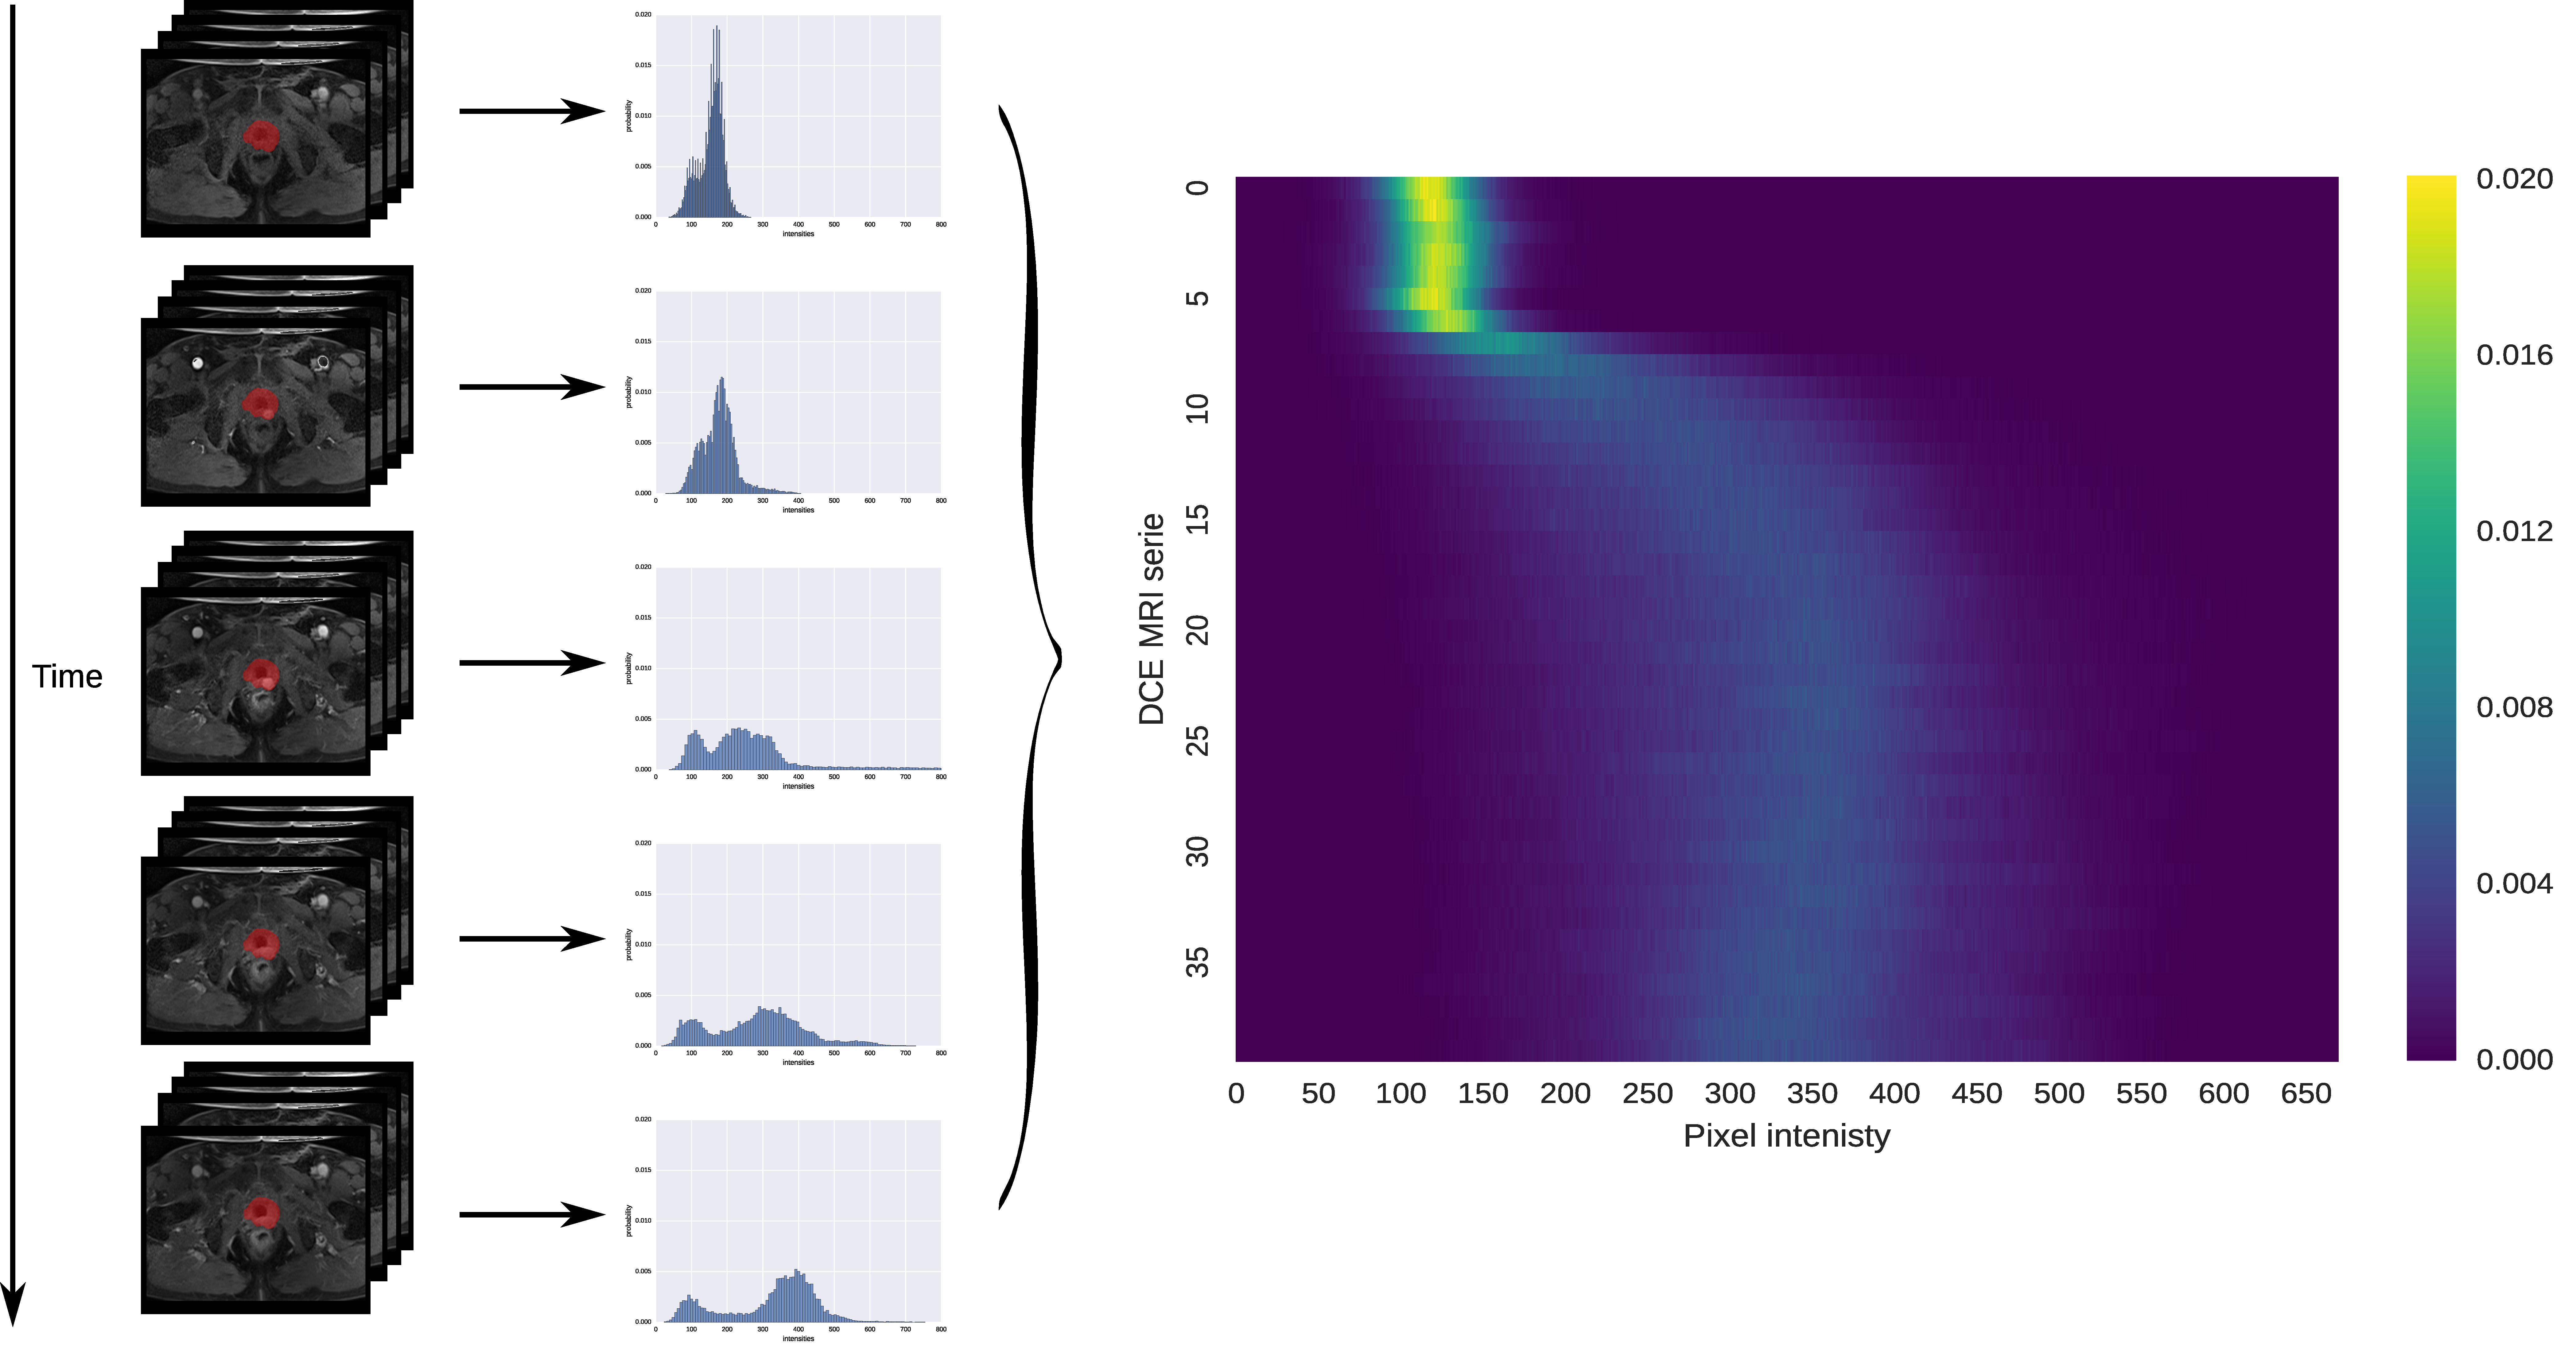
\includegraphics[width=1\textwidth]{images/DCE-normalization/heatmaprep.pdf}} \hfill
  \hspace*{\fill}
  \\
  \hspace*{\fill}
  \subfigure[$I_0$: 117; $t_0$: 6\textsuperscript{th} serie; wider st. dev.]{\label{subfig:pat1}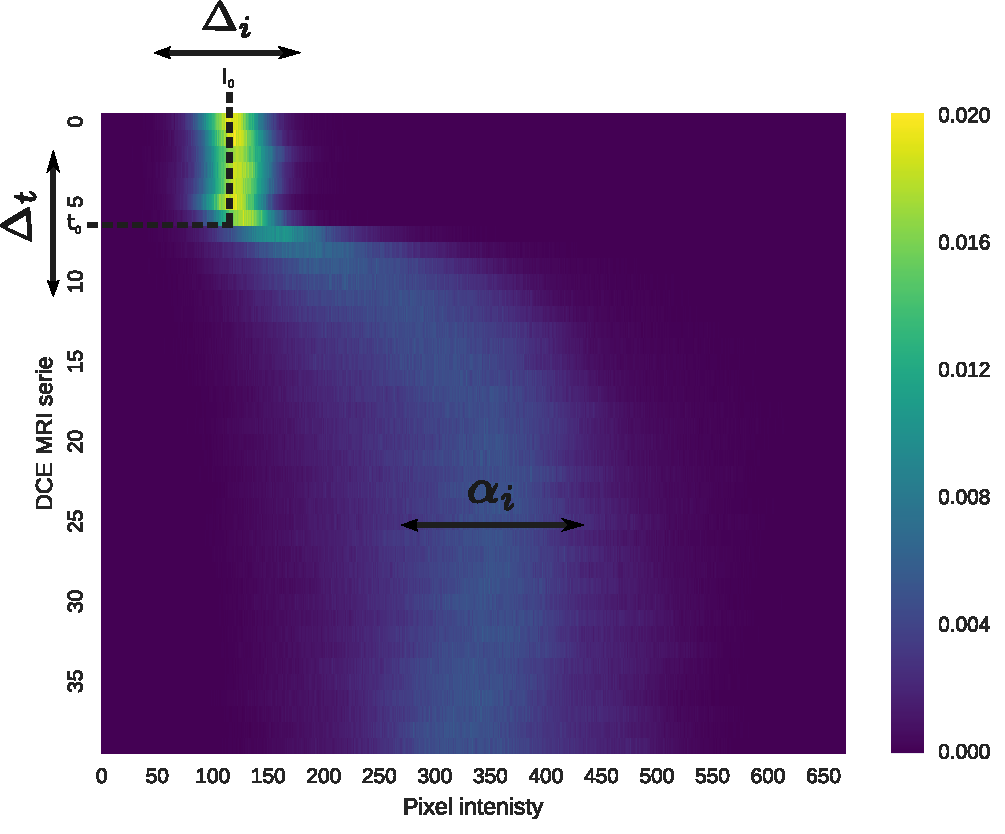
\includegraphics[width=.49\textwidth]{images/DCE-normalization/pat1_annotated.pdf}} \hfill
  \subfigure[$I_0$: 103; $t_0$: 4\textsuperscript{th} serie; narrower std. dev.]{\label{subfig:pat2}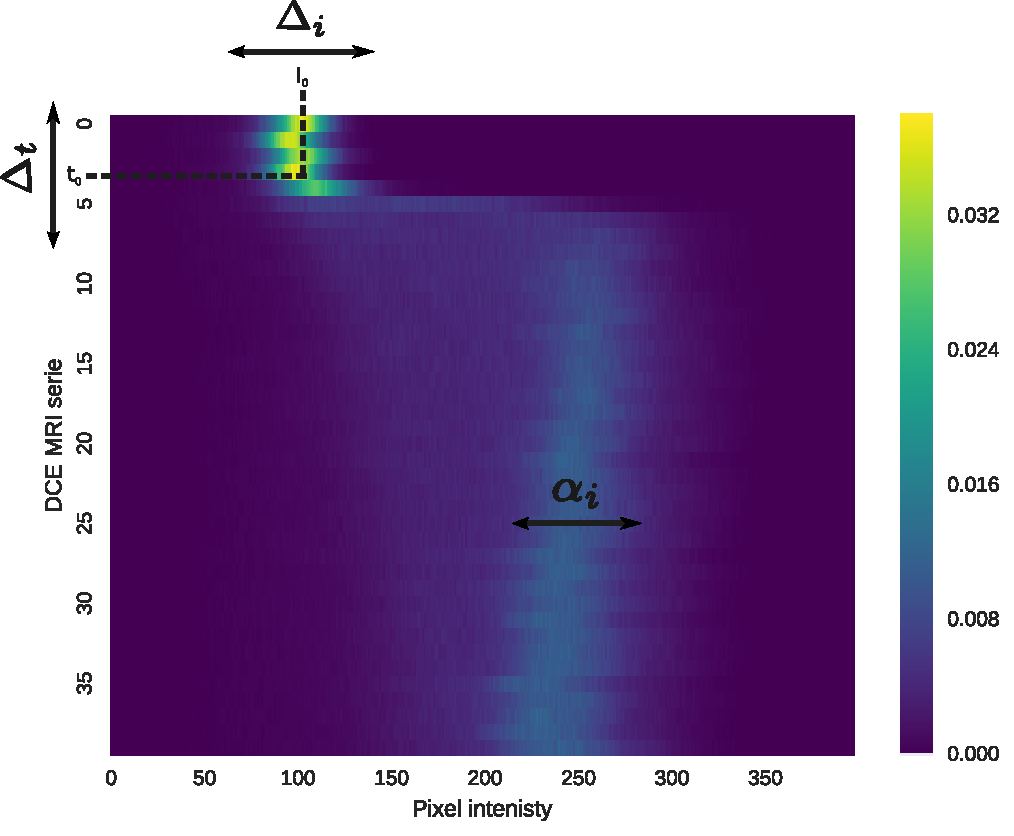
\includegraphics[width=.49\textwidth]{images/DCE-normalization/pat2_annotated.pdf}} \hfill
  \hspace*{\fill}
  \caption{\textbf{Overview of the normalization applied to \ac{dce}-\ac{mri}
      modality.} \protect\subref{subfig:pathhist} Illustration of the heatmap
    representation: all \ac*{pdf}s of the prostate gland are concatenated together
    to build an heatmap; \protect\subref{subfig:pat1}-\protect\subref{subfig:pat2}
    Heatmap of 2 patients revealing the three types of inter-patient variations:
    intensity shift ($\Delta_i$), time shift ($\Delta_t$), and intensity scale
    ($\alpha_i$).}
  \label{fig:heatmap}
\end{figure*}

\subparagraph{Normalization of \ac{dce}-\ac{mri}} In \ac{dce}-\ac{mri}, the
intensity \ac{pdf} of the prostate gland does not follow a unique type of
distribution such as Rician or Gaussian distribution, as shown in
Fig.\,\ref{subfig:pathhist}. Indeed, the inter-patient variations are more
complex due to the temporal acquisition. A better means of observing these
variations is to represent the intensity \ac{pdf} of the prostate gland over
time--- requiring segmentation of the prostate ---using a heatmap
representation as shown in Fig.\,\ref{subfig:pathhist}. By analyzing this
heatmap representation across patients (see Fig.\,\ref{subfig:pat2}), the
following variations are highlighted: (i) intensity offsets ($\Delta_i$) of the
\ac{pdf} peak, (ii) a time offset ($\Delta_t$) depending on the contrast agent
arrival, and (iii) a change of scale ($\alpha_i$) related to the signal
enhancement. Therefore, our normalization method should attenuate all of these
variations and be performed globally across the different time sequences rather
than for each independent sequence.

\begin{figure}
  \centering
  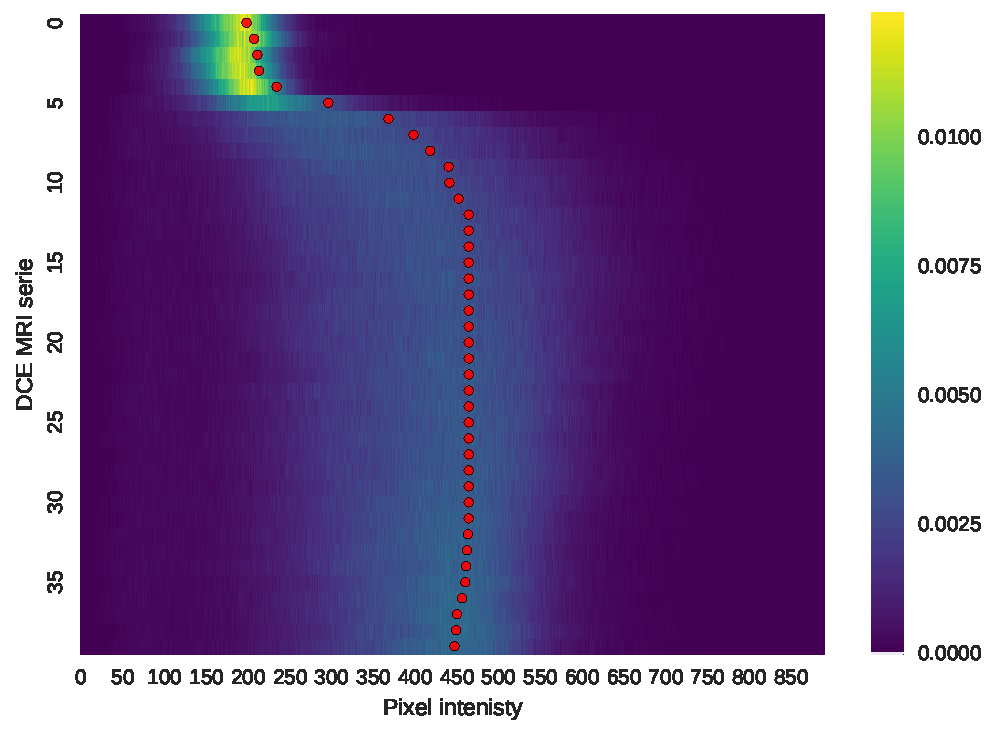
\includegraphics[width=0.8\linewidth]{images/DCE-normalization/estimator.pdf}
  \caption{\textbf{Estimation of $\Delta_i$.} This estimate is found by using
    the shortest-path through the graph $\mathcal{G}$.}
  \label{fig:estimator}
\end{figure}

\subparagraph{Graph-based intensity offsets correction} Before standardizing
each sequence, the first step of the normalization process is to cancel the
intensity shift specific at each patient, which occurs due to the media
injection. As previously mentioned, the intensity \ac{pdf} does not always
follow a Rician or a Gaussian distribution over time in
\ac{dce}-\ac{mri}. Therefore, the mean of these distributions cannot be used as
a potential estimate for these offsets. Additionally, these offsets should be
characterized by a smooth transition between series over time.

Thus, this problem is solved using graph approach: considering the intensity
\ac{pdf} over time as shown in Fig.\,\ref{subfig:pathhist}, the offsets
correspond to the boundary splitting, the heatmap into two partitions such that
they are as close as possible to the peak of the intensity \ac{pdf} (see
Fig.\,\ref{fig:estimator} for an illustration). Given the heatmap, a directed
weighted graph $\mathcal{G}=(\mathcal{V}, \mathcal{E})$ is built by taking each
bin---, i.e., the probability for a given time and pixel intensity---, of the
heatmap as a node and connecting each pair of bins by an edge. The edge weight
$w_{ij}$ between two nodes $i$ and $j$ corresponds to two pixel intensities at
positions $(x_i, y_i)$ and $(x_j, y_j)$, respectively, is defined as in
Eq.\,\eqref{eq:weight}, as follows:

\begin{equation}\small
  w_{ij} = \begin{cases}
    \alpha \exp(1 - \frac{H(i)}{\max(H)})       & \text{if } x_j = x_i + 1 \text{ and } y_j = y_i, \\
    (1 - \alpha) \exp(1 - \frac{H(i)}{\max(H)}) & \text{if } x_j = x_i \text{ and } y_j = y_i + 1, \\
    0                                           & \text{otherwise},
  \end{cases}
  \label{eq:weight}
\end{equation}

\noindent where $H$ is the heatmap, and $\alpha$ is a smoothing parameter
controlling for the partitioning.

Therefore, these offsets related to $\Delta_i$ are estimated by finding the
shortest-path to cross the graph using Dijkstra's algorithm.  The entry and
exiting nodes are set to be the bin with the maximum probability for the first
value in the \ac{dce}-\ac{mri} series and the bin corresponding to the median
value for the last value of the \ac{dce}-\ac{mri} series, respectively.  To
ensure a robust estimation of these offsets, the process of finding the
shortest-path is repeated by shifting the data and updating the heatmap as well
as the graph $\mathcal{G}$. The procedure is stopped once the offset found does
not change. In general, this process is not repeated more than 3 times.  The
parameter $\alpha$ is set to $0.9$, empirically. Figure~\ref{fig:estimator}
illustrates the final estimation of the offsets, $\Delta_i$ (i.e., red
landmark), found for each value of the \ac{dce}-\ac{mri} series. Therefore,
each intensity offset is subtracted for each \ac{dce}-\ac{mri}.

\begin{figure*}
  \centering
  \hspace*{\fill}
  \subfigure[]{\label{fig:rmse}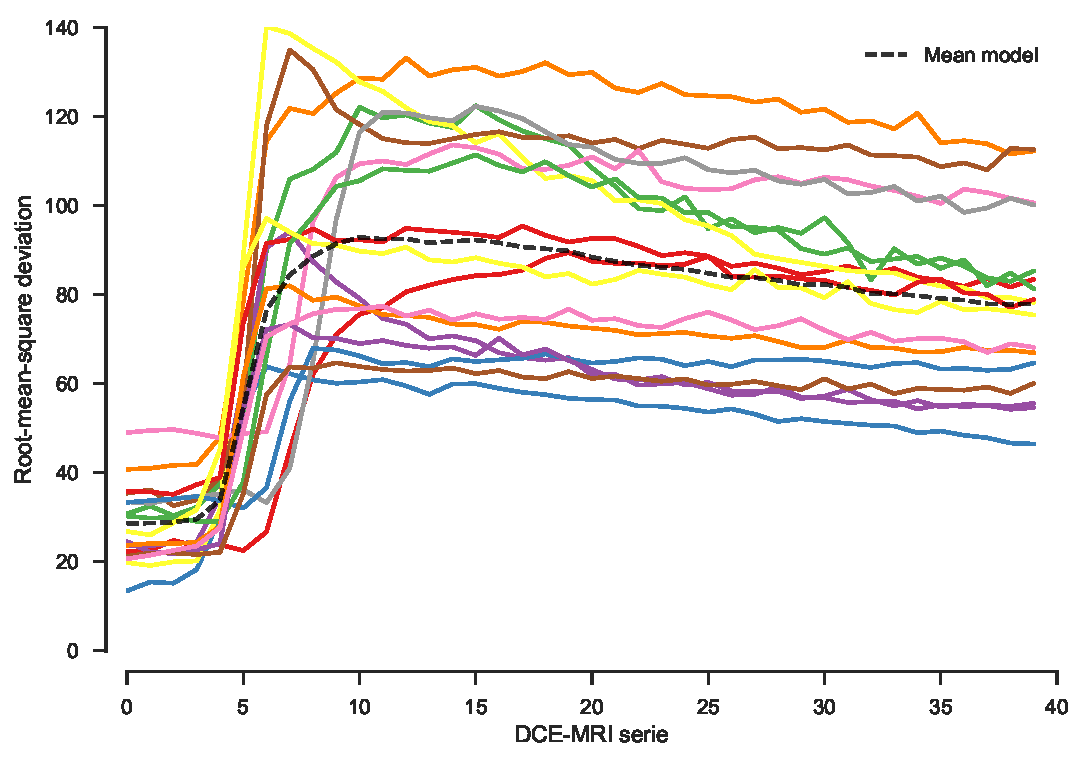
\includegraphics[width=.44\textwidth]{images/DCE-normalization/rmse.pdf}} \hfill
  \subfigure[]{\label{fig:rmseal}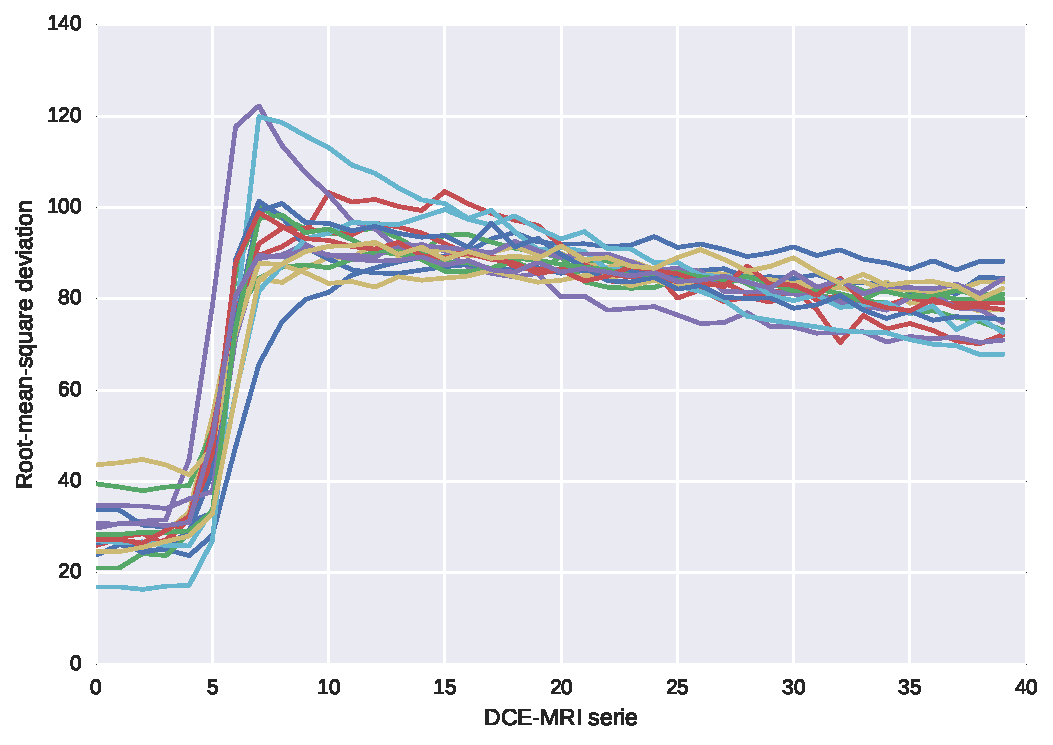
\includegraphics[width=.49\textwidth]{images/DCE-normalization/rmse_aligned.pdf}}
  \hspace*{\fill}
  \caption{\textbf{Correction of the time offset and the data
    dispersion.} \protect\subref{fig:rmse} \acs*{rmse} computed for each
  patient of our dataset; \protect\subref{fig:rmseal} \acs*{rmse} after alignment using the curve parametric model.}
  \label{fig:curveal}
\end{figure*}

\subparagraph{Time offset and data dispersion correction} The next variations
to correct are the time offset, $\Delta_t$, and the data dispersion,
$\alpha_i$. By computing the \ac{rmse} of the intensities for each value of the
\ac{dce}-\ac{mri} series, one can observe these two variations as shown in
Fig.\,\ref{fig:rmse}. Therefore, these variations are corrected by registering
the \ac{rmse} of each patient to a mean model computed using all patients and
obtaining an estimate for the parameters $\Delta_t$ and $\alpha_i$. An
illustration of the correction applied to each \ac{rmse} of the patients is
shown in Fig.\,\ref{fig:rmseal}. Once all of these parameters have been
determined, the data are shifted and scaled.

\subsubsection{\ac{mrsi} features}\label{features:mrsi}

First, the \ac{mrsi} signal is pre-processed by correcting the
phase~\cite{Chen2002}, baseline~\cite{xi2008baseline}, and
frequency~\cite{Parfait2012} shifts. Additionally, each \ac{mrsi} spectrum is
normalized using the L$_2$ norm, which has been shown to be the most efficient
normalization method in \ac{mrsi}~\cite{Parfait2012}.  Once the signal are
pre-processed, two strategies are commonly used to extract discriminative
features from \ac{mrsi}: (i) relative quantification based on metabolite
quantification and (ii) spectra extraction~\cite{Parfait2012}.

In \emph{relative quantification}, the relative concentration of the
metabolites of interest (i.e. citrate and choline) is computed by robustly
fitting and integrating the peak(s). Therefore, the relative
concentrations of citrate and choline are quantified using a Gaussian
mixture. We solve this problem with a non-linear curve fitting problem under
constraints. The constraints imposed are related to the peak location of the
citrate and choline.

The latter strategies is based on the work of~\cite{Parfait2012}. The full
\ac{mrsi} signal from \SIrange{2}{4}{\ppm} is used as features, letting the
classifier selecting the relevant \si{\ppm} bandwidth of interest.

Similarly to the \ac{dce}-\ac{mri} data, a set of experiment is designed in
\acs{sec}\,\ref{exp:dce_mrsi_sel} to select the most discriminative approach.

\subsection{Data balancing}\label{features:balancing}

Imbalanced dataset is a recurrent issue in classification. A dataset is
imbalanced when a class is over-represented compared to other classes. In our
application, the number of cancerous voxels is under-represented compared to
healthy voxels. In classification, imbalanced datasets are either under- or
over-sampled ahead of training, avoiding the classifiers to learn a bias toward
the over-represented class. In this section, we present the different methods
which we used to alleviate this issue. The reader is referred to
\acs{sec}\,\ref{exp:balancing} presenting the experiments investigating the
effect of balancing the dataset during the training phase.

\subsubsection{\Acl*{us1}}

A dataset can be balanced by \ac{us1} samples from the over-represented
classes.

\Ac{nm} offers three different methods to under-sample the majority
class~\cite{mani2003knn}. In \ac{nm1}, samples from the majority class are
selected such that for each sample, the average distance to the $k$ \ac{nn}
samples from the minority class is minimum. \ac{nm2} diverges from \ac{nm1} by
considering the $k$ farthest neighbours samples from the minority class. In
\ac{nm3}, a subset $M$ containing samples from the majority class is generated
by finding the $m$ \ac{nn} from each sample of the minority class. Then,
samples from the subset $M$ are selected such that for each sample, the average
distance to the $k$ \ac{nn} samples from the minority class is maximum. In our
experiment, $k$ and $m$ are fixed to 3.

\Ac{iht} select samples with a high hardness
threshold~\cite{smith2014instance}. Hardness indicates the likelihood of
mis-classification rate for each samples. The notation of instance hardness
are drawn through the decomposition of $p(h \vert t)$ using Bayes' theorem,
where $h$ represent the mapping function used to map input features to their
corresponding labels and $t$ represents the training set.
\begin{equation}
  IH_h(\langle x_{i}, y_{i}\rangle) = 1 - p(y_i \vert x_i, h).\
  \label{eq:iht}
\end{equation}
Therefore, under-sampling is performed by keeping the most probable samples ---
i.e, filtering the samples with high hardness value --- through \ac{kcv}
training sets while considering specific threshold for filtering.

\subsubsection{\Acl*{os}}

In contrast to \ac{us1} techniques, a dataset can be balanced by \ac{os} the
samples from the under-represented class.

\Ac{smote} is a method to generate new synthetic
samples~\cite{chawla2002smote}. Let define $x_i$ as a sample belonging to the
minority class. Let define $x_{nn}$ as a randomly selected sample from the
$k$-\ac{nn} of $x_i$, with $k$ set to 3. A new sample $x_j$ is generated such
that $x_j = x_i + \sigma \left( x_{nn} - x_i \right)$, where $\sigma$ is a
random number in the interval $\left[0,1\right]$. \Ac{smoteb1} over-samples the
minority class samples similarly to \ac{smote}~\cite{han2005borderline}.
However, instead of using all the minority samples, it focuses on the
borderline samples of minority class.  Borderline samples simply indicate the
samples that are closer to the other class. First, the borderline samples of
minority class are detected. A sample $x_{i}$ belongs to borderline samples if
more than half of its $k$-\ac{nn} samples belong to the majority
class. Synthetic data is then created based on \ac{smote} method for borderline
samples, by selecting. Then, $s$-\ac{nn} of the minority class are selected to
generate synthetic sample similarly to \ac{smote}. \Ac{smoteb2} performs
similarly to \ac{smoteb1}~\cite{han2005borderline}.  However, the $s$-\ac{nn}
are not computed by only considering the minority class but by considering both
classes. The same generation rules as \ac{smote} is used.

\subsection{Feature selection}\label{features:selection}

Tree-based models can be efficiently used to find which set of features is the
most discriminative by using the Gini importance. In a tree classifier, the
Gini impurity criterion of the child nodes is inferior to the parent node. For
each individual feature, adding the decrease of the Gini impurity along the
tree gives information about the feature importance: the higher, the
better. Therefore, one can add the decrease of the Gini impurity across all the
trees of a forest and obtain the importance of a specific feature for this
forest. Subsequently, the $K$ most important features are selected to perform
the feature selection.

Therefore, in addition to use \ac{rf} as our base classifier, we also use it to
identified important features as reported by the experiments in
\acs{sec}\,\ref{exp:selection}.

\subsection{Classification}

\ac{rf} serves as our base classifier. The use of \ac{rf} is motivated since
that it leads to the best performance in the state-of-the-art
methods~\cite{Litjens2014,lemaitre2015computer}. The number of trees in
ensemble is set to 100.

\subsection{Model validation}

All experiments use a \ac{lopo} to report the results of the different models.

\subsection{Computationally aspects}

For reproducibility, we rely on the Python ecosystem:
NumPy~\cite{walt2011numpy}, SciPy~\cite{jones2014scipy},
scikit-learn~\cite{pedregosa2011scikit},
imbalanced-learn~\cite{lemaitre2017imbalanced},
scikit-image~\cite{van2014scikit},
and mahotas~\cite{coelho2012mahotas}. The registration is performed using
ITK~\cite{ibanez2005itk}. We further provide all source code of all
experiments\footnote{\url{https://github.com/I2Cvb/mp-mri-prostate}} with the
associated
dataset\footnote{\url{https://zenodo.org/record/162231#.W3AAMBh9hhE}}.

\begin{figure*}
  \hspace*{\fill}
  \subfigure[] {
    \label{fig:dce_roc}
    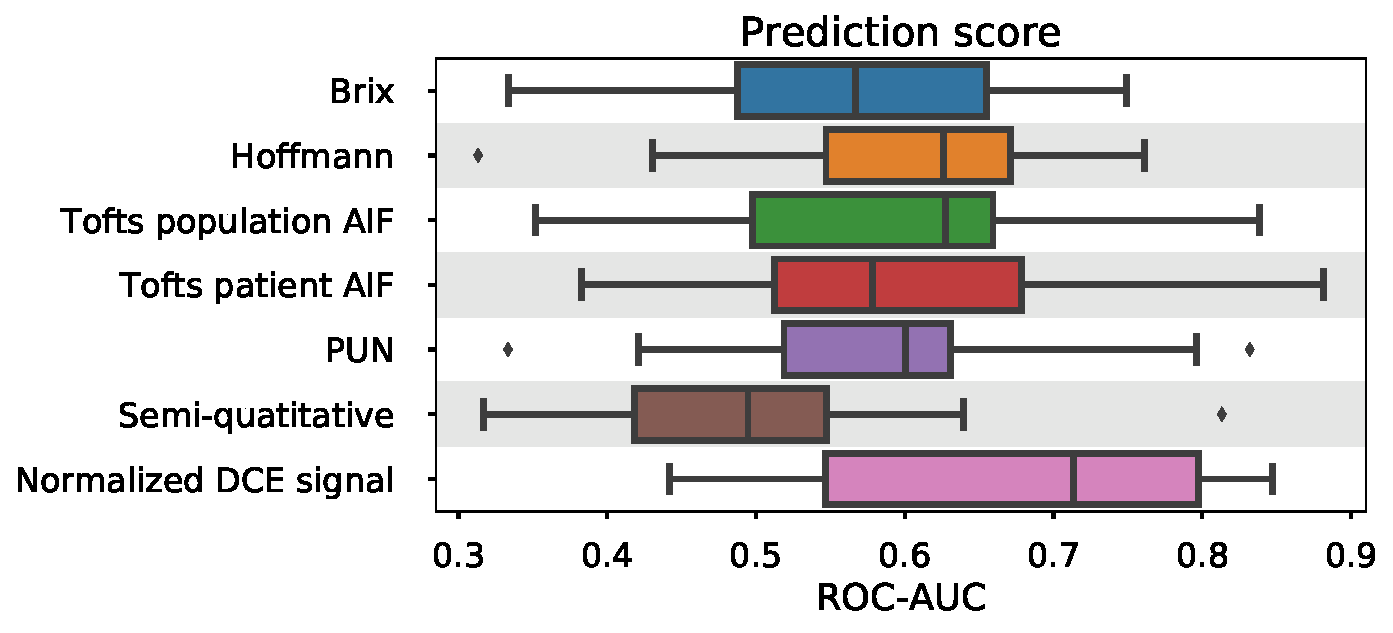
\includegraphics[width=.4\textwidth]
    {images/box_plot_dce.pdf}
  }
  \hfill
  \subfigure[] {
    \label{fig:mrsi_roc}
    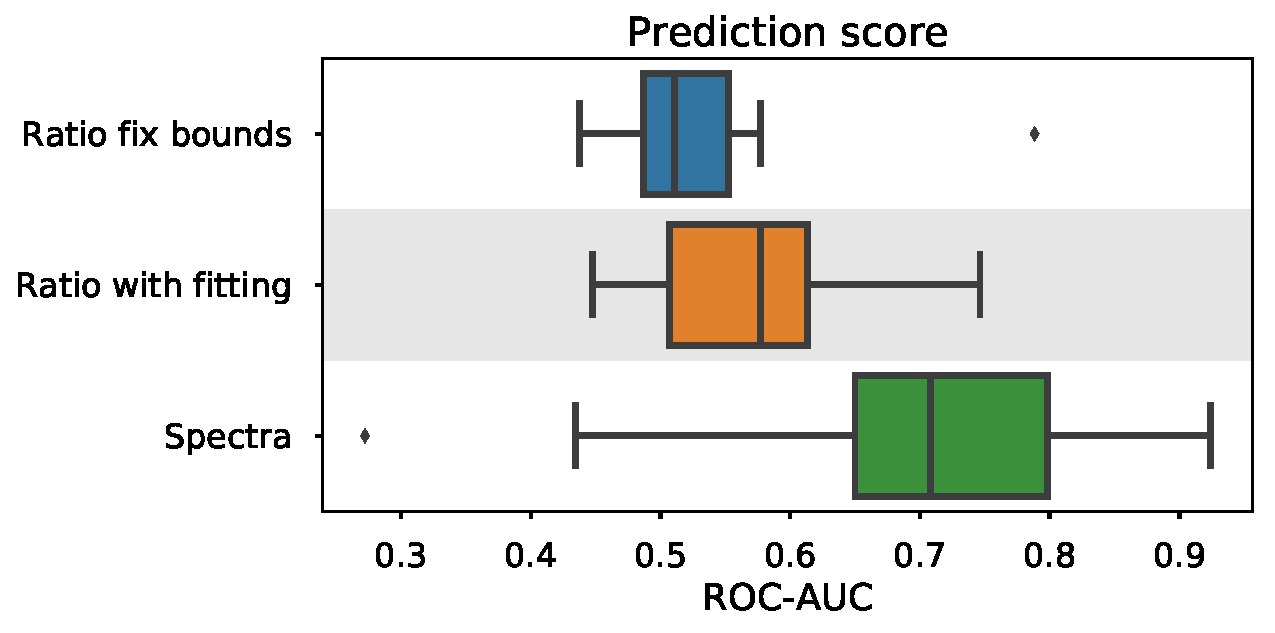
\includegraphics[width=.35\textwidth]
    {images/box_plot_mrsi.pdf}
  }
  \hspace*{\fill}
  \caption[]{\textbf{Impact of the features used with the \ac{dce}-\ac{mri} and
    \ac{mrsi}.} \protect\subref{fig:dce_roc} Comparison of the different
  quantitative and semi-quantitative models in \ac{dce}-\ac{mri};
  \protect\subref{fig:mrsi_roc} comparison of quantification approaches in
  \ac{mrsi}.}
  \label{fig:dce_results}
\end{figure*}

\begin{figure*}
  \hspace*{\fill}
  \subfigure[]{
    \label{fig:feat_imp_t2w}
    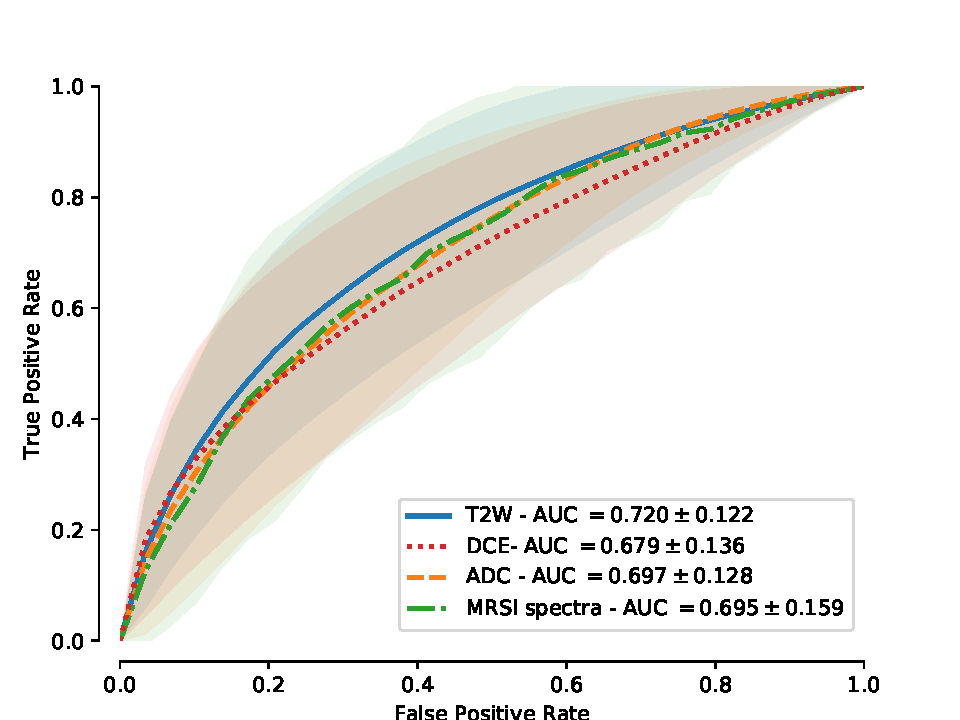
\includegraphics[width=.35\textwidth]
    {images/all.pdf}
  }
  \hfill
  \subfigure[] {
    \label{fig:boxplot_modalities}
    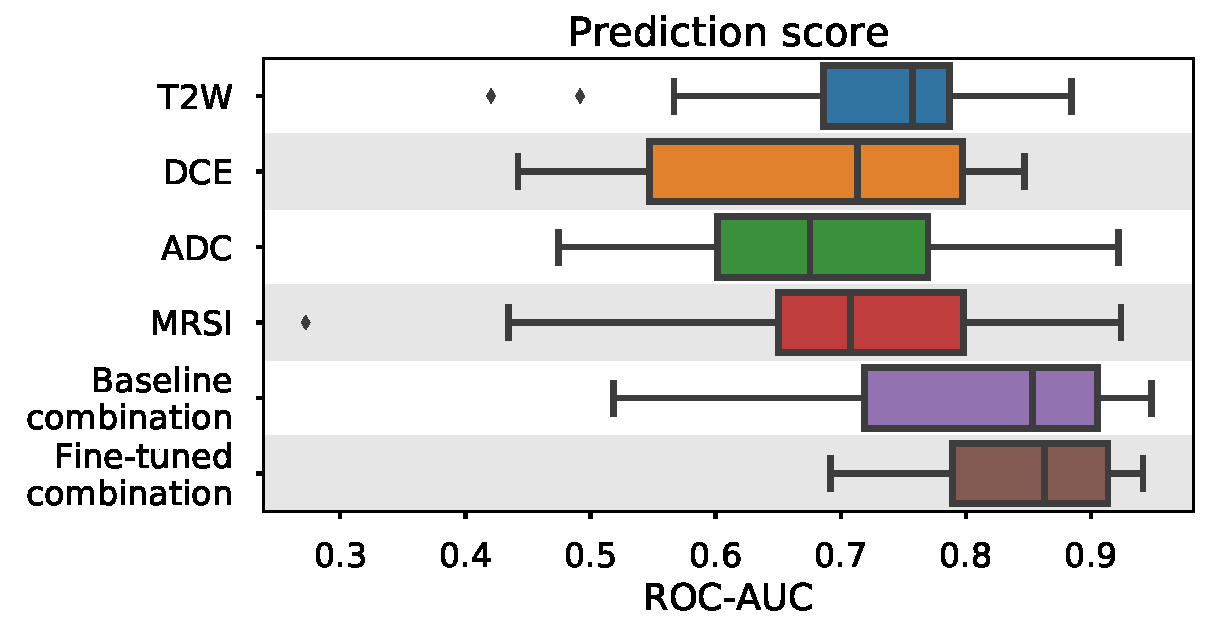
\includegraphics[width=.45\textwidth]
    {images/box_plot_all.pdf}
  }
  \hspace*{\fill}
  \caption[]{\textbf{Comparison of discriminative power of different
      strategies.} We investigate the baseline classification performance of
    each modality. In addition, we explore the combination of the those
    modalities and check the effect of fine tuning the machine learning model
    learned.}
  \label{fig:summary_single_modality}
\end{figure*}

\section{Experiment and results}\label{sec:experiments}

\subsection{Data}\label{sec:data}

The \ac{mpmri} data are acquired from a cohort of patients with
higher-than-normal level of \ac{psa}.  The acquisition is performed using a
\SI{3}{\tesla} whole body \ac{mri} scanner (Siemens Magnetom Trio TIM,
Erlangen, Germany) using sequences to obtain \ac{t2w}-\ac{mri},
\ac{dce}-\ac{mri}, \ac{dw}-\ac{mri}, and \ac{mrsi}.  Aside of the \ac{mri}
examination, these patients also have undergone a guided-biopsy.  The dataset
is composed of a total of 19 patients of which 17 patients have biopsy proven
\ac{cap} and 2 patients are ``healthy'' with negative biopsies.  From those 17,
12 patients have a \ac{cap} in the \ac{pz}, 3 patients have \ac{cap} in the
\ac{cg}, 2 patients have invasive \ac{cap} in both \ac{pz} and \ac{cg}.  An
experienced radiologist has segmented the prostate organ --- on
\ac{t2w}-\ac{mri}, \ac{dce}-\ac{mri}, and \ac{adc}-\ac{mri} --- as well as the
prostate zones --- i.e., \ac{pz} and \ac{cg} ---, and \ac{cap} on the
\ac{t2w}-\ac{mri}.

A \SI{3}{\mm} slice fat-suppressed \ac{t2w} fast spin-echo sequence (\ac{tr}:
\SI{3400}{\ms}, \ac{te}: \SI{85}{\ms}, \ac{etl}:13) is used to acquire images
in sagittal and oblique coronal planes, the latter planes being orientated
perpendicular or parallel to the prostate \ac{pz} – rectal wall axis.
Three-dimensional \ac{t2w} fast spin-echo (\ac{tr}: \SI{3600}{\ms}, \ac{te}:
\SI{143}{\ms}, \ac{etl}: 109, slice thickness: \SI{1.25}{\mm}) images are then
acquired in an oblique axial plane.  The nominal matrix and \ac{fov} of the 3D
\ac{t2w} fast spin-echo images are
\SI[product-units=repeat]{320x256}{\milli\metre\squared} and
\SI[product-units=repeat]{280x240}{\milli\metre\squared}, respectively, thereby
affording sub-millimetric pixel resolution within the imaging plane.

\ac{dce}-\ac{mri} is performed using a fat suppressed 3D T$_1$ VIBE sequence
(\ac{tr}: \SI{3.25}{\ms},\ac{te}: \SI{1.12}{\ms}, Flip angle:\SI{10}{\degree};
Matrix: $256 \times 192$; \ac{fov}: $280 \times 210$ (with \SI{75}{\percent}
rectangular \ac{fov}); slab of 16 partitions of \SI{3.5}{\mm} thickness;
temporal resolution: \SI{6}{\s}/slab over approximately \SI{5}{\minute}).  A
power injector (Medrad, Indianola, USA) is used to provide a bolus injection of
Gd-DTPA (Dotarem, Guerbet, Roissy, France) at a dose of \SI{0.2}{\ml}
Gd-DTPA/kg of body weight.

\ac{dw}-\ac{mri} images have been acquired using the single-shot spin-echo
echo-planar imaging (EPI) technique.  As proposed by
Stejskal\,\emph{et~al.}~\cite{stejskal1965spin}, the diffusion-encoding
gradients have been applied using a pulsed gradient spin-echo technique
resulting in diffusion images acquired at 2 b-values --- i.e.,
\SI{100}{\second\per\milli\meter\squared} and
\SI{800}{\second\per\milli\meter\squared} --- and in the 3 orthogonal
directions.  Sequential sampling of the k-space has been used with a \ac{te} of
\SI{101}{\ms}, a \ac{tr} of \SI{4200}{\ms}, and a bandwidth of
\SI{1180}{\hertz\per\px}.  Other parameters included a \ac{fov} of
\SI{240}{\milli\metre}, an acquisition matrix size of $128 \times 128$ and a
slice thickness of \SI{3.5}{\milli\metre}.  The \ac{adc} map has been directly
generated by the Siemens workstation from the raw data on a pixel-by-pixel
basis.

\ac{mrsi} is performed using a water and lipid suppressed double-spin-echo
point-resolved spectroscopic (PRESS) sequence optimized for quantification
detection of choline and citrate metabolites.  Water and lipid have been
suppressed using a dual-band spectral spatial pulse technique.  In order to
eliminate signals from adjacent tissues, especially periprostatic lipids and
the rectal wall up to 8 outer voxel saturation pulses have been used.  Datasets
have been acquired as $16 \times 12 \times 16$ --- interpolated to $16 \times
16 \times 16$ phase-encoded spectral arrays, a \ac{te} of \SI{140}{\ms}, a
\ac{tr} of \SI{720}{\ms} and \SI{13}{\minute} of acquisition time.  A spectral
bandwidth of \SI{1250}{\hertz} has been used with 512 data points.  A
combination of an elliptic weighted averaged k-space acquisition scheme 3D
filtering of the signal in k-space have been used, the latter in order to
reduce intervoxel signal combination.  Shimming has been carried out using the
Siemenbens 3D Mapshim routine on a voxel adapted to the volume of the entire
prostate gland.  Additional unsuppressed water acquisitions at \ac{te} of
\SI{30}{\ms}, \SI{80}{\ms}, and \SI{140}{\ms} of \SI{1.5}{\minute} have also
been performed in order to allow quantification with respect to prostate water.
Systematic verification of the global shim --- i.e., over the complete 3D
PRESS-selected volume --- revealed line widths at half-height of the water peak
of the order of \SIrange{20}{30}{\hertz}, routinely.  The line widths for
individual voxels are of the order of \SIrange{8}{12}{\hertz}.  The total
examination time, including the time spent positioning the patient, is
approximately 45 minutes.

\begin{figure*}
  \hspace*{\fill}
  \subfigure[]{
    \label{fig:feat_imp_t2w}
    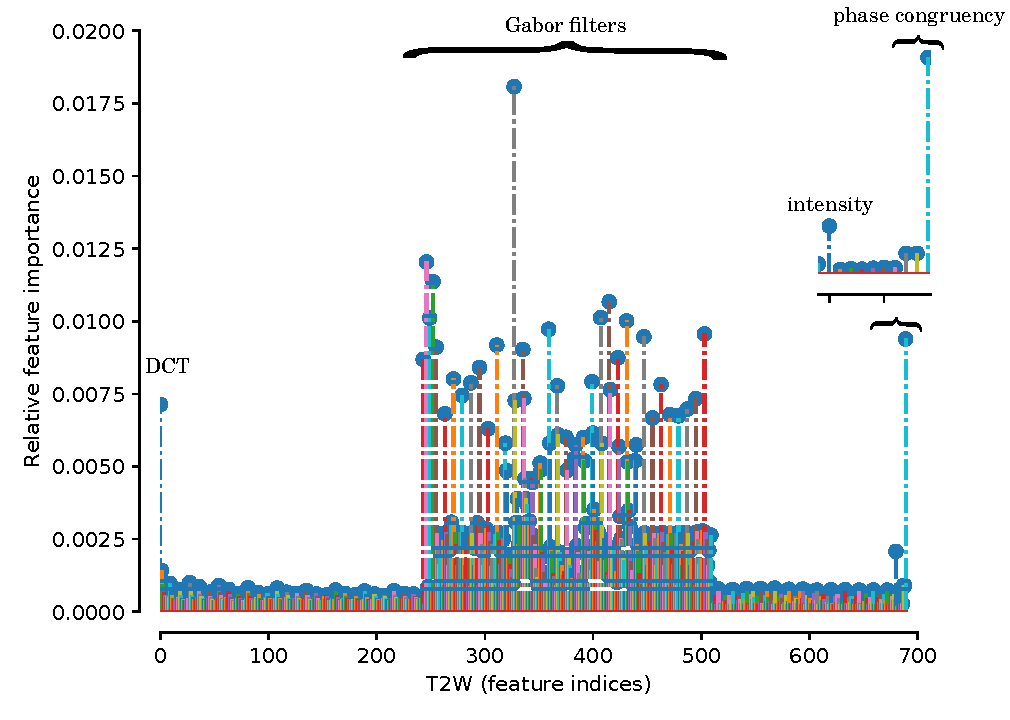
\includegraphics[width=.45\textwidth]
    {images/feature_importance/feature_importance_t2w_annotated.pdf}
  }
  \hfill
  \subfigure[] {
    \label{fig:feat_imp_adc}
    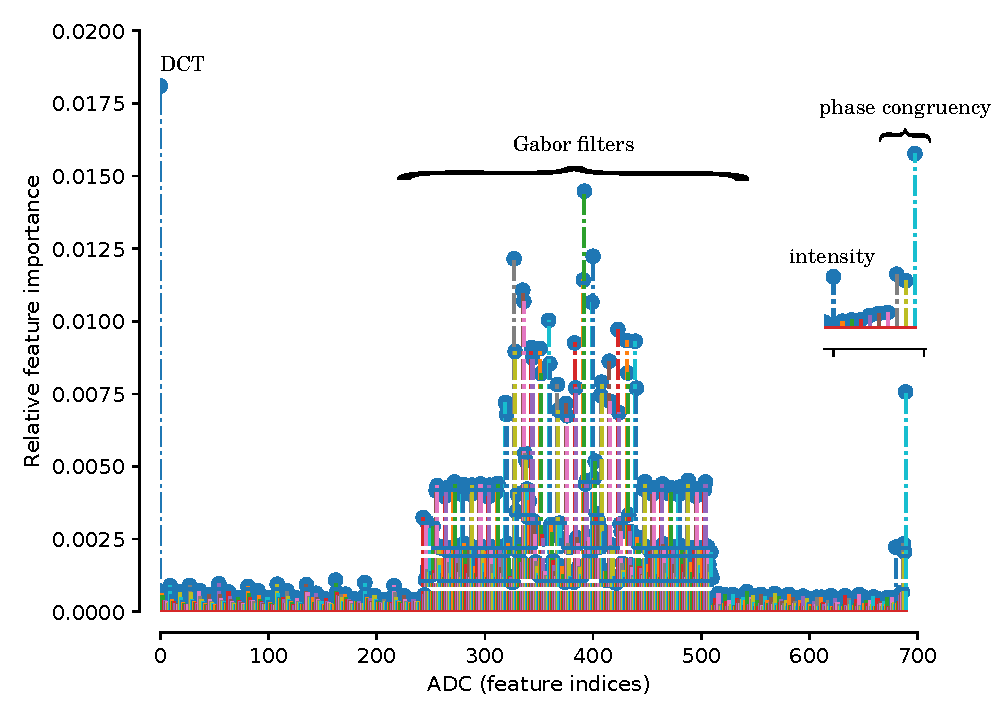
\includegraphics[width=.45\textwidth]
    {images/feature_importance/feature_importance_adc_annotated.pdf}
  }
  \hspace*{\fill}\\
  \hspace*{\fill}
  \subfigure[] {
    \label{fig:feat_imp_dce}
    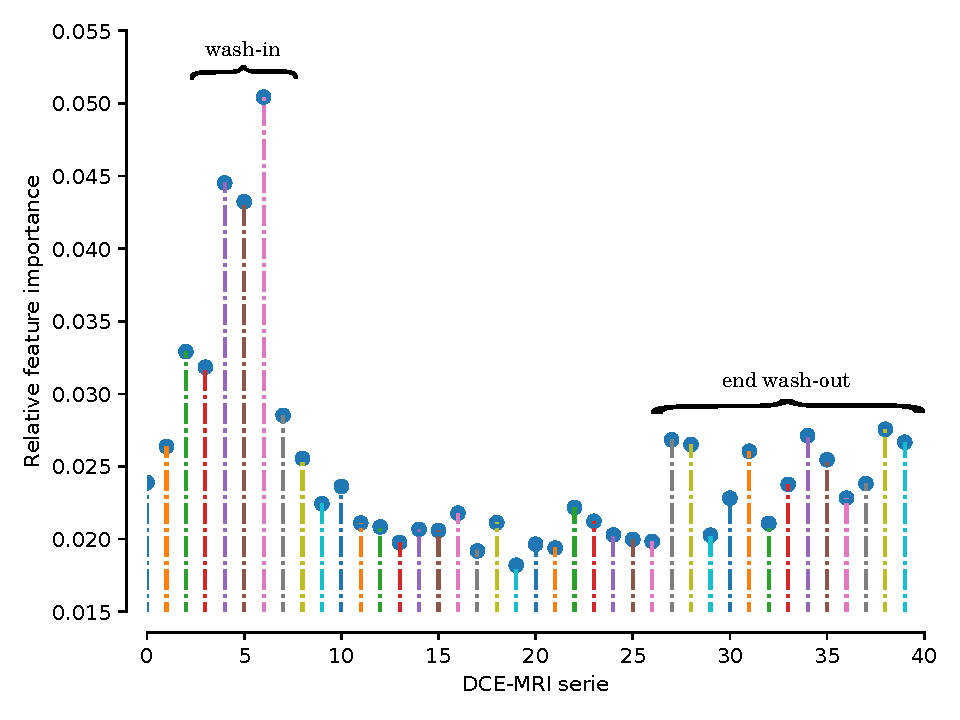
\includegraphics[width=.45\textwidth]
    {images/feature_importance/feature_importance_dce_annotated.pdf}
  }
  \hfill
  \subfigure[]{
    \label{fig:feat_imp_mrsi}
    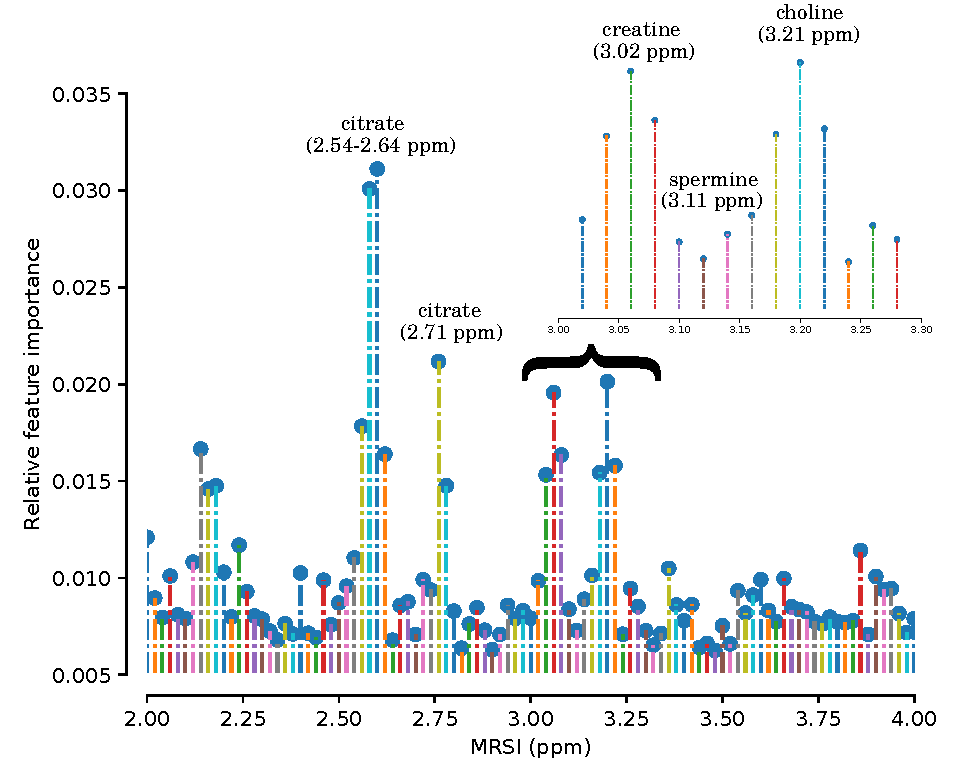
\includegraphics[width=.45\textwidth]
    {images/feature_importance/feature_importance_mrsi_annotated.pdf}
  }
  \hspace*{\fill}
  \caption[]{\textbf{Feature importance.} We explore the relative features
    importance found by a \ac{rf} classifier on each modality.}
  \label{fig:feat_importance}
\end{figure*}

\subsection{Selection of the feature detection strategies for
  \ac{dce}-\ac{mri} and \ac{mrsi}}\label{exp:dce_mrsi_sel}

As presented in \acs{sec}\,\ref{features:dce} and \ref{features:mrsi}, several
methods exists to extract information from \ac{dce}-\ac{mri} and \ac{mrsi}
modalities. These features are redundant and only one of the model/strategy
should be selected. Therefore, this experiment intend to compare the
induced performance of these features and select the best one.

The methods presented in \acs{sec}\,\ref{features:dce} --- i.e. (i) Brix
model~\cite{brix1991pharmacokinetic}, (ii) Hoffman
model~\cite{hoffmann1995pharmacokinetic}, (iii) Tofts
model~\cite{tofts1995quantitative}, (iv) \ac{pun}
model~\cite{gliozzi2011phenomenological}, (v) semi-quantitative
approach~\cite{huisman2001accurate}, and (vi) use of the normalized \ac{dce}
signal --- are extracted. The performance of each strategy is reported in
\acs{fig}\,\ref{fig:dce_roc} in terms of \ac{roc}-\ac{auc}. Using the entire
normalized \ac{dce} signal strategy outperforms the other approaches with an
\ac{auc} of $0.679 \pm 0.136$.

As presented in \acs{sec}\,\ref{features:mrsi}, 3 strategies are used to
extract features from the \ac{mrsi} modality: (i) compute the ratio of the
citrate concentration over the choline concentration where the concentrations
are determined with fixed \si{\ppm} bounds, (ii) compute the ratio of the
citrate concentration over the choline concentration where the concentrations
are determined by fitting the peaks, and (iii) using a part of the \ac{mrsi}
signal containing the choline and citrate peaks. The performance of each
strategy is highlighted in the \acs{fig}\,\ref{fig:mrsi_roc}. Similarly to the
\ac{dce}-\ac{mri} experiment, using the entire signal lead to the best
performance with a \ac{roc}-\ac{auc} of $0.695 \pm 0.159$.

\subsection{Classification baselines}

\Acl{fig}~\ref{fig:summary_single_modality} summarizes the classification
performance for each individual modality as well as their
combinations. Features extracted on the \ac{t2w}-\ac{mri} modality are the most
discriminative leading to a \ac{roc}-\ac{auc} of $0.720 \pm 0.122$. Features
from \ac{adc} and \ac{mrsi} modalities achieve similar performance,
i.e. $0.697 \pm 0.128$ and $0.695 \pm 0.159$, respectively. Finally, the
\ac{dce}-\ac{mri} modality is the less discriminative modality with a
\ac{roc}-\ac{auc} of $0.679 \pm 0.136$. In a clinical setting, those results
would be considered as almost ``acceptable'' (i.e. \ac{roc}-\ac{auc} ranging
from 0.7 to 0.8~\cite{hosmer2004applied}). Combining all features together
improve the \ac{roc}-\ac{auc} to $0.802 \pm 0.130$ which is considered as
``excellent'' level of discrimination (i.e. \ac{roc}-\ac{auc} ranging
from 0.8 to 0.9~\cite{hosmer2004applied}).

\subsection{Effect of fine tuning}

To further improve the results, we propose to correct the problem of imbalanced
classes by applying some over- and under-sampling technique during the
training. In addition, we propose to select a subset of the most relevant
features.

\subsubsection{Data balancing}\label{exp:balancing}

\begin{figure}
  \centering
  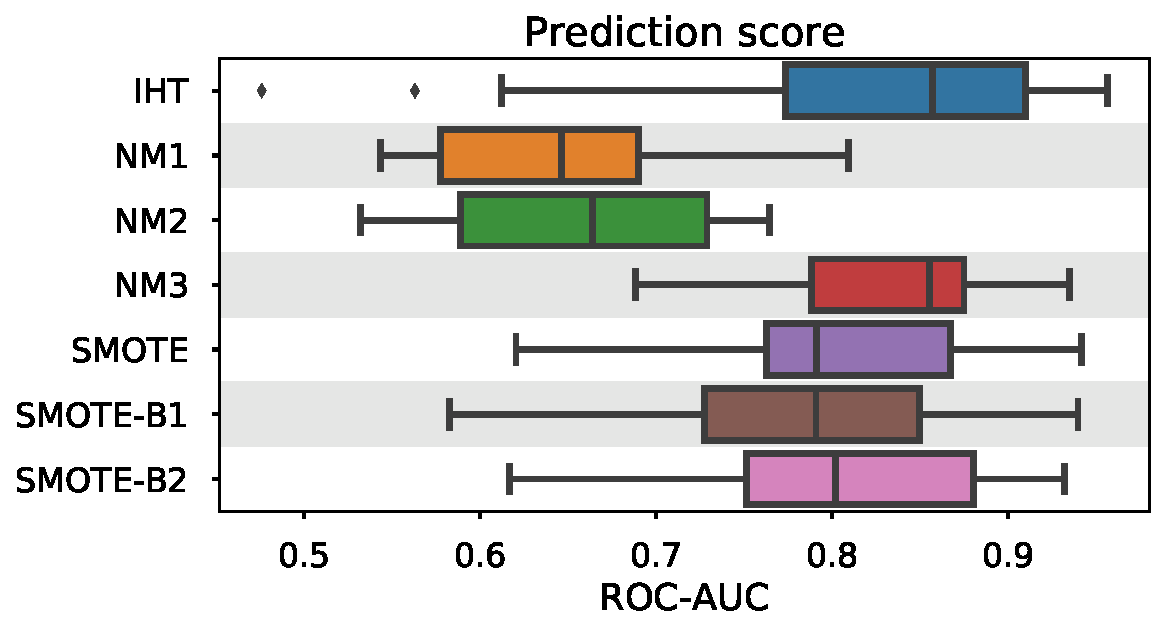
\includegraphics[width=0.8\linewidth]{images/box_plot_balancing_all.pdf}
  \caption[Balancing]{\textbf{Effect of data balancing.} \ac{roc}-\ac{auc}
    obtained with the different balancing strategies.}
  \label{fig:balancing}
\end{figure}

We empirically check which of the methods presented in
\acs{sec}\,\ref{features:balancing} leads to the best classification
performance. The results are reported in \acs{fig}\,\ref{fig:balancing}. In
conclusion, \Ac{nm3} leads to the best performance with a \ac{roc}-\ac{auc} of
$0.824 \pm 0.076$.

\subsubsection{Feature selection}\label{exp:selection}

\begin{table}
  \caption{\textbf{Feature selection.} Number and type of features selected for
  each individual modality.}
  \centering
  \scriptsize
  \begin{tabular}{llll}
    \toprule
    \multicolumn{1}{c}{\textbf{\acs*{t2w}-\acs*{mri}}} & \multicolumn{1}{c}{\textbf{\acs*{adc}}} & \multicolumn{1}{c}{\textbf{\acs*{dce}-\acs*{mri}}} & \multicolumn{1}{c}{\textbf{\acs*{mrsi}}} \\
    \midrule
    113 Gabor filters & 53 Gabor filters & 14 samples  & 78 samples \\
    1 phase congruency & 2 phase congruency & & \\
    4 edges & & & \\
    1 intensity & & & \\
    \midrule
    \multicolumn{4}{c}{\textbf{267 features}} \\
    \bottomrule
  \end{tabular}
  \label{tab:selfeatocc}
\end{table}

The combination of the features from all modalities lead to a potential
correlation between features. In addition, some features might not be
discriminative and there is no benefit to include them in the model
trained. Therefore, we propose to select a subset of features which are found
to be the most important using the approach presented in
\acs{sec}\,\ref{features:selection}. \Acl{tab}~\ref{tab:selfeatocc} summarizes
the number and type of features which are selected. To complement this table,
\acs{fig}\,\ref{fig:feat_importance} highlights the relative feature importance
of each feature found by the \ac{rf} classifier.

In the image-based modalities --- i.e. \ac{t2w}-\ac{mri} and \ac{adc} --- the
Gabor features, \ac{dct}, phase congruency, and intensity are considered
particularly relevant. In the \ac{mrsi} modality, the \si{ppm} bands found
relevant are associated with the citrate, creatine, and choline while in the
\ac{dce}-\ac{mri}, the wash-in and the end of the wash-out corresponds to the
time points considered as important.

\subsubsection{Fine-tuned classifier performance}\label{exp:classification}

\begin{figure}
  \hspace*{\fill}
  \subfigure[\acs*{auc} = 0.922]{\label{fig:pat634}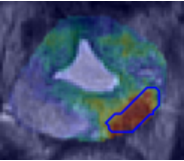
\includegraphics[height=.1\textheight]{images/qualitative_results/patient_634_roi.pdf}}
  \hfill
  \subfigure[\acs*{auc} =
  0.914]{\label{fig:pat1036}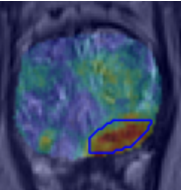
\includegraphics[height=.1\textheight]{images/qualitative_results/patient_1036_roi.pdf}}
  \hspace*{\fill}\\
  \hspace*{\fill}
  \subfigure[\acs*{auc} = 0.692]{\label{fig:pat634}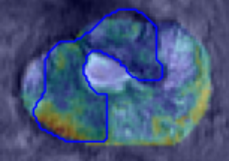
\includegraphics[height=.1\textheight]{images/qualitative_results/patient_410_roi.pdf}}
  \hfill
  \subfigure[\acs*{auc} = 0.735]{\label{fig:pat1036}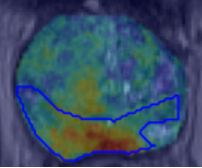
\includegraphics[height=.1\textheight]{images/qualitative_results/patient_1041_roi.pdf}}
  \hspace*{\fill}
  \caption[]{\textbf{Qualitative results.} Detection of our \acs*{mpmri}
    \acs*{cad} for \acs*{cap} detection. The blue contours corresponds to the
    \ac{cap} while the \texttt{jet} overlay represents the probability.}
  \label{fig:resultcad}
\end{figure}

We finally trained a fine-tuned \ac{rf} classifier on the subset of features
found relevant and by applying the \ac{nm3} under-sampling. The classification
performance in terms of \ac{roc}-\ac{auc} is reported in
\acs{fig}\,\ref{fig:summary_single_modality}. The fine tuning of the classifier
allows to improve the performance from $0.802 \pm 0.130$ to $0.836 \pm 0.083$.
\Acl{fig}~\ref{fig:resultcad} shows some example of \ac{cap} segmentation.

\subsection{Effect of including \acs*{mrsi} modality}\label{discussion:mrsi}

\begin{figure}
  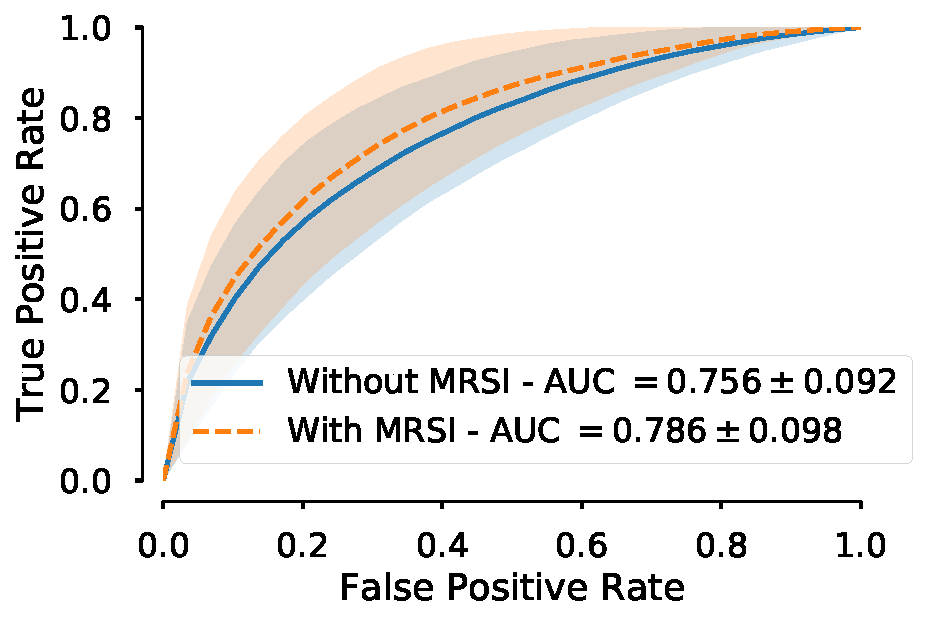
\includegraphics[width=.45\textwidth]{images/stacking_wt_mrsi.pdf}
  \caption{\textbf{Effect of including \ac{mrsi} modality.} \ac{roc}-\ac{auc}
    by plug-in/-out \ac{mrsi} modality.}
  \label{fig:stacking_mrsi}
\end{figure}

We can recall that \ac{mrsi} has nearly never been used together with the other
modalities --- i.e., \ac{t2w}-\ac{mri}, \ac{dce}-\ac{mri}, and \ac{adc} map ---
apart of the recent work of
Trigui\,\emph{et~al.}~\cite{trigui2016classification,trigui2017automatic}.
Therefore, we propose in this experiment to compare the classification
performance by removing the \ac{mrsi} features and observed the effect of
including this modality.

In this regard, we propose to train 2 models such that one of the model will
omit the \ac{mrsi} modality. Therefore, we use a stacking approach for which
the first layer is composed of a classifier (a \ac{rf} classifier) for each
input modality and a second layer with a single classifier (a \ac{gb}
classifier) to aggregate the predictions of the first layer. Therefore, 2
stacking classifiers are trained: (i) the first model uses 4 base
classifiers in its first layer while (ii) the second model uses 3 base
classifiers in its first layer, omitting the classifier for the \ac{mrsi}
modality.

As in all other experiments, a \ac{lopo} validation scheme is used and the
results obtained from \ac{roc} analysis are depicted in
\acs{fig}\,\ref{fig:stacking_mrsi}. Thus, including \ac{mrsi} into the
classification pipeline increases the \ac{auc} from $0.756 \pm 0.092$ to $0.786
\pm 0.098$ highlighting the gain of incorporating the \ac{mrsi} modality in the
\ac{cad} system.

\section{Discussions}\label{sec:conclusion}



\bibliographystyle{elsarticle-num} 
\bibliography{literature_review_2}

\end{document}

%  LocalWords:  voxels
